\documentclass{exam}

\usepackage{siunitx} 
\usepackage{graphicx}
\usepackage[fleqn]{amsmath}
\usepackage{cancel}
\usepackage{float}
\usepackage{mdwlist}
\usepackage{booktabs}
\usepackage{cancel}
\usepackage{polynom}
\usepackage{caption}
\usepackage{fullpage}
\usepackage{xfrac}
\usepackage{enumerate}

\newcommand{\degree}{\ensuremath{^\circ}} 
\everymath{\displaystyle}

% \begin{figure}[H]
%   \centering
%   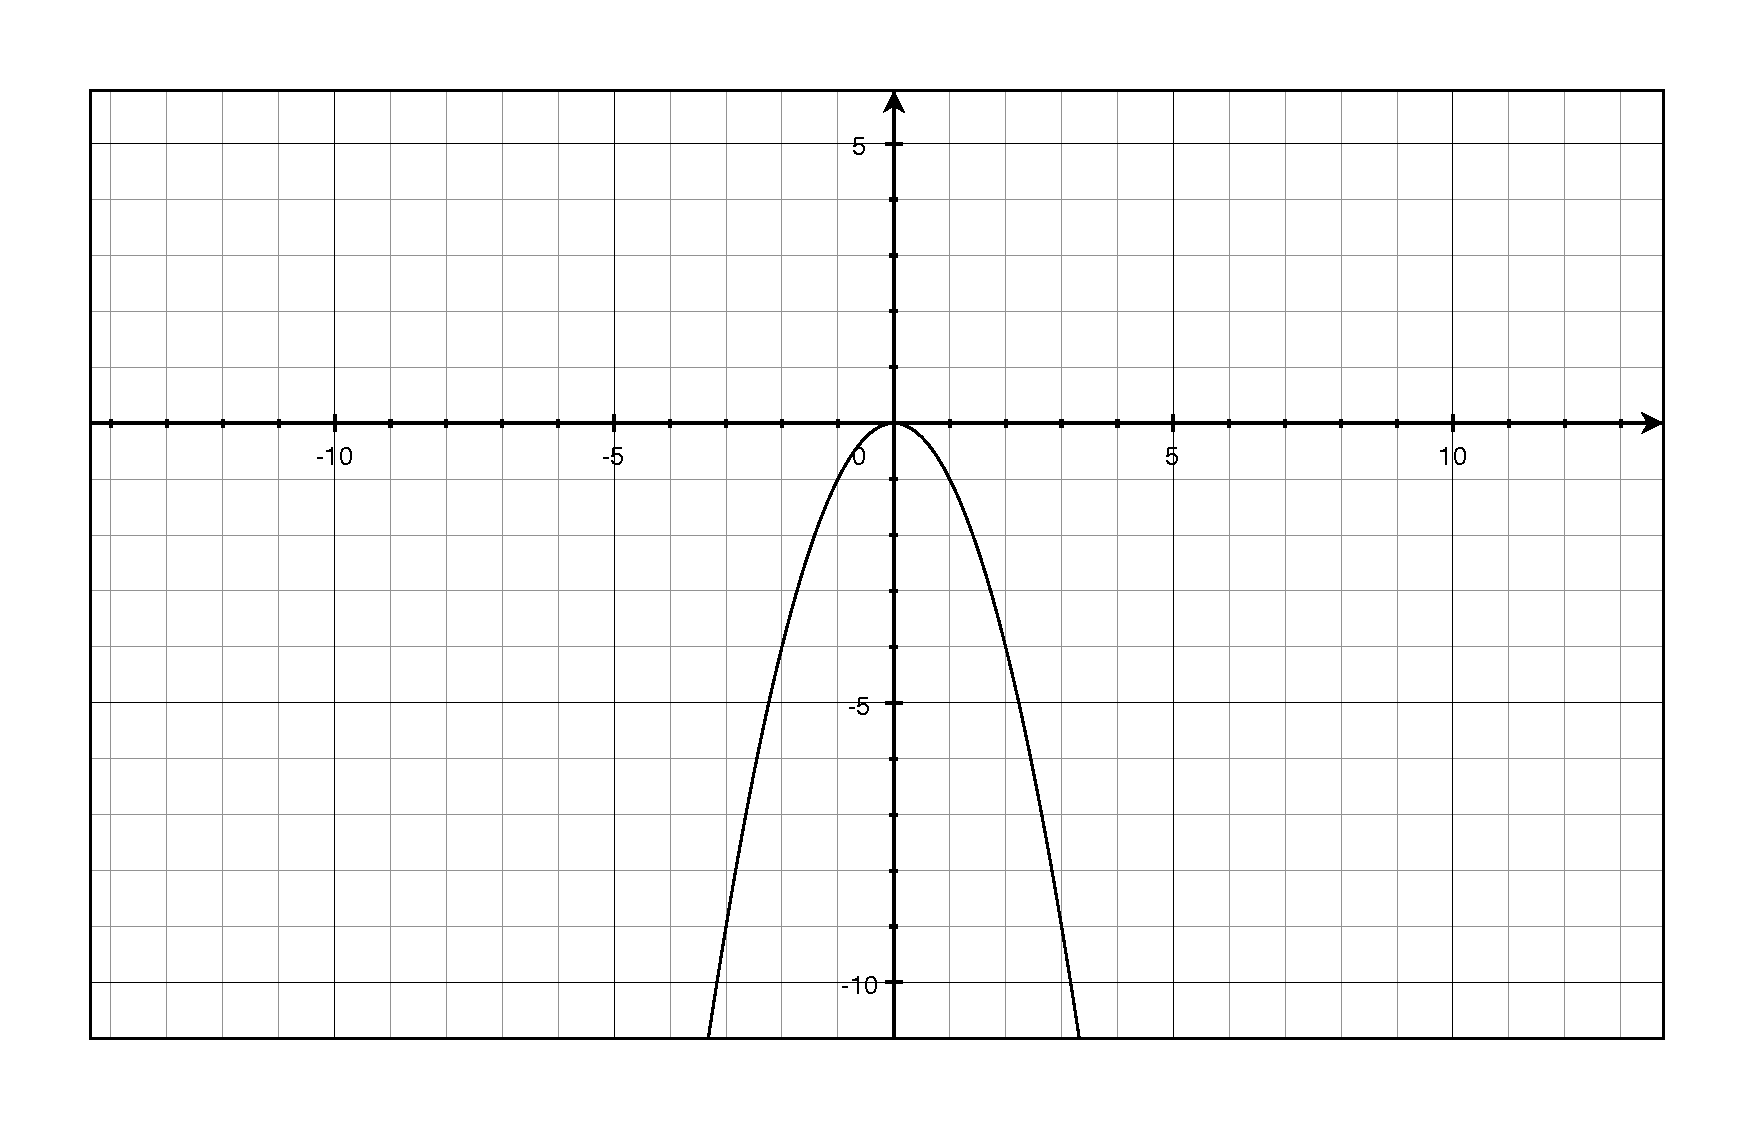
\includegraphics[scale=.3]{problem7.eps}
%   \caption*{Problem 7}
% \end{figure}

% \begin{tabular}{cc}
% \toprule
% period & amplitude \\
% \midrule
%   $\pi$ & $2$ \\
% \bottomrule
% \end{tabular}

\printanswers

\ifprintanswers 
  \usepackage{2in1, lscape} 
\fi

\author{}
\date{January 23, 2013}
\title{Math 141 \\ Homework 3}

\begin{document}

\maketitle

\section{Homework}

\begin{itemize*}
  \item Read Section 2.4
  \item Section 2.4: 1-18, 21, 27-40, 47-48, 61-63, 69-70, 73
\end{itemize*}

\section{Extra Credit}
Section 2.4, problems 75-77.

\ifprintanswers
  \pagebreak

  \begin{description}
    \item[75]
      If $f$ and $g$ are both even, $f(-x) = f(x)$ and $g(-x) = g(x)$.  
      \begin{align*}
        (f + g)(-x) &= f(-x) + g(-x) \\
          &= f(x) + g(x) \\
          &= (f + g)(x) \\
      \end{align*}
      So in this case, $(f + g)(x)$ is even.

      If $f$ and $g$ are both odd, $f(-x) = -f(x)$ and $g(-x) = -g(x)$.  
      \begin{align*}
        (f + g)(-x) &= -f(x) + (-g(x)) \\
          &= - (f(x) + g(x)) \\
          &= -(f + g)(x) \\
      \end{align*}
      So in this case, $(f + g)(x)$ is odd.

      If $f$ is even and $g$ is odd, $f(-x) = f(x)$ and $g(-x) = -g(x)$.  
      \begin{align*}
        (f + g)(-x) &= f(x) + (-g(x)) \\
          &= f(x) - g(x) \\
      \end{align*}
      So in this case, $(f + g)(x)$ is neither even nor odd.

    \item[76]
      If $f$ and $g$ are both even, $f(-x) = f(x)$ and $g(-x) = g(x)$.  
      \begin{align*}
        (f \cdot g)(-x) &= f(-x) \cdot g(-x) \\
          &= f(x) \cdot g(x) \\
          &= (f \cdot g)(x) \\
      \end{align*}
      So in this case, $(f \cdot g)(x)$ is even.

      If $f$ and $g$ are both odd, $f(-x) = -f(x)$ and $g(-x) = -g(x)$.  
      \begin{align*}
        (f \cdot g)(-x) &= -f(x) \cdot (-g(x)) \\
          &= f(x) \cdot g(x) \\
          &= (f \cdot g)(x) \\
      \end{align*}
      So in this case, $(f \cdot g)(x)$ is even.

      If $f$ is even and $g$ is odd, $f(-x) = f(x)$ and $g(-x) = -g(x)$.  
      \begin{align*}
        (f \cdot g)(-x) &= f(x) \cdot (-g(x)) \\
          &= - f(x) \cdot g(x) \\
      \end{align*}
      So in this case, $(f \cdot g)(x)$ is odd.

    \item[77]
      If $n$ is even, the function is even and if $n$ is odd the function is odd.

  \end{description}

  \pagebreak

  \section{Section 2.4}

  \begin{description}
    \item[1] 
      \begin{parts}
        \part shift down 5
        \part shift right 5
      \end{parts}

    \item[2] 
      \begin{parts}
        \part shift left 7
        \part shift up 7
      \end{parts}

    \item[3] 
      \begin{parts}
        \part shift left $\sfrac{1}{2}$
        \part shift up $\sfrac{1}{2}$
      \end{parts}

    \item[4] 
      \begin{parts}
        \part reflect around x-axis
        \part reflect around y-axis
      \end{parts}

    \item[5] 
      \begin{parts}
        \part reflect around x-axis and stretch by a factor of 2 in the vertical direction
        \part reflect around x-axis and shrink by a factor of $\sfrac{1}{2}$ in the vertical direction
      \end{parts}

    \item[6] 
      \begin{parts}
        \part reflect around y-axis and shift up 5
        \part stretch by a factor of three in the vertical direction and shift down 5
      \end{parts}

    \item[7] 
      \begin{parts}
        \part shift right 4 and up $\sfrac{3}{4}$.
        \part shift left 4 and down $\sfrac{3}{4}$.
      \end{parts}

    \item[8] 
      \begin{parts}
        \part shift left 2, shift down 2, and stretch by a factor of 2 in the vertical direction
        \part shift right 2, shift up 2, and stretch by a factor of 2 in the vertical direction
      \end{parts}

    \item[9] 
      \begin{parts}
        \part shrink by a factor of $\sfrac{1}{4}$ in the horizontal direction
        \part stretch by a factor of 4 in the horizontal direction
      \end{parts}

    \item[10] 
      \begin{parts}
        \part shrink by a factor of $\sfrac{1}{2}$ in the horizontal direction and reflect around the y-axis
        \part shrink by a factor of $\sfrac{1}{2}$ in the horizontal direction and shift down 1.
      \end{parts}

    \item[11] $g(x) = (x - 2)^2$

    \item[12] $g(x) = x^3 + 3$

    \item[13] $g(x) = |x + 1| + 2$

    \item[14] $g(x) = |2x|$

    \item[15] $g(x) = - \sqrt{x + 2}$

    \item[16] $g(x) = - (x - 2)^2 + 1$

    \item[17]
      \begin{parts}
        \part 3
        \part 1
        \part 2
        \part 4
      \end{parts}

    \item[18]
      \begin{parts}
        \part 2
        \part 3
        \part 1
        \part 4
      \end{parts}

    \item[21]
      \begin{parts}
        
        \part $f(x) = \frac{1}{x}$
          \begin{figure}[H]
            \centering
            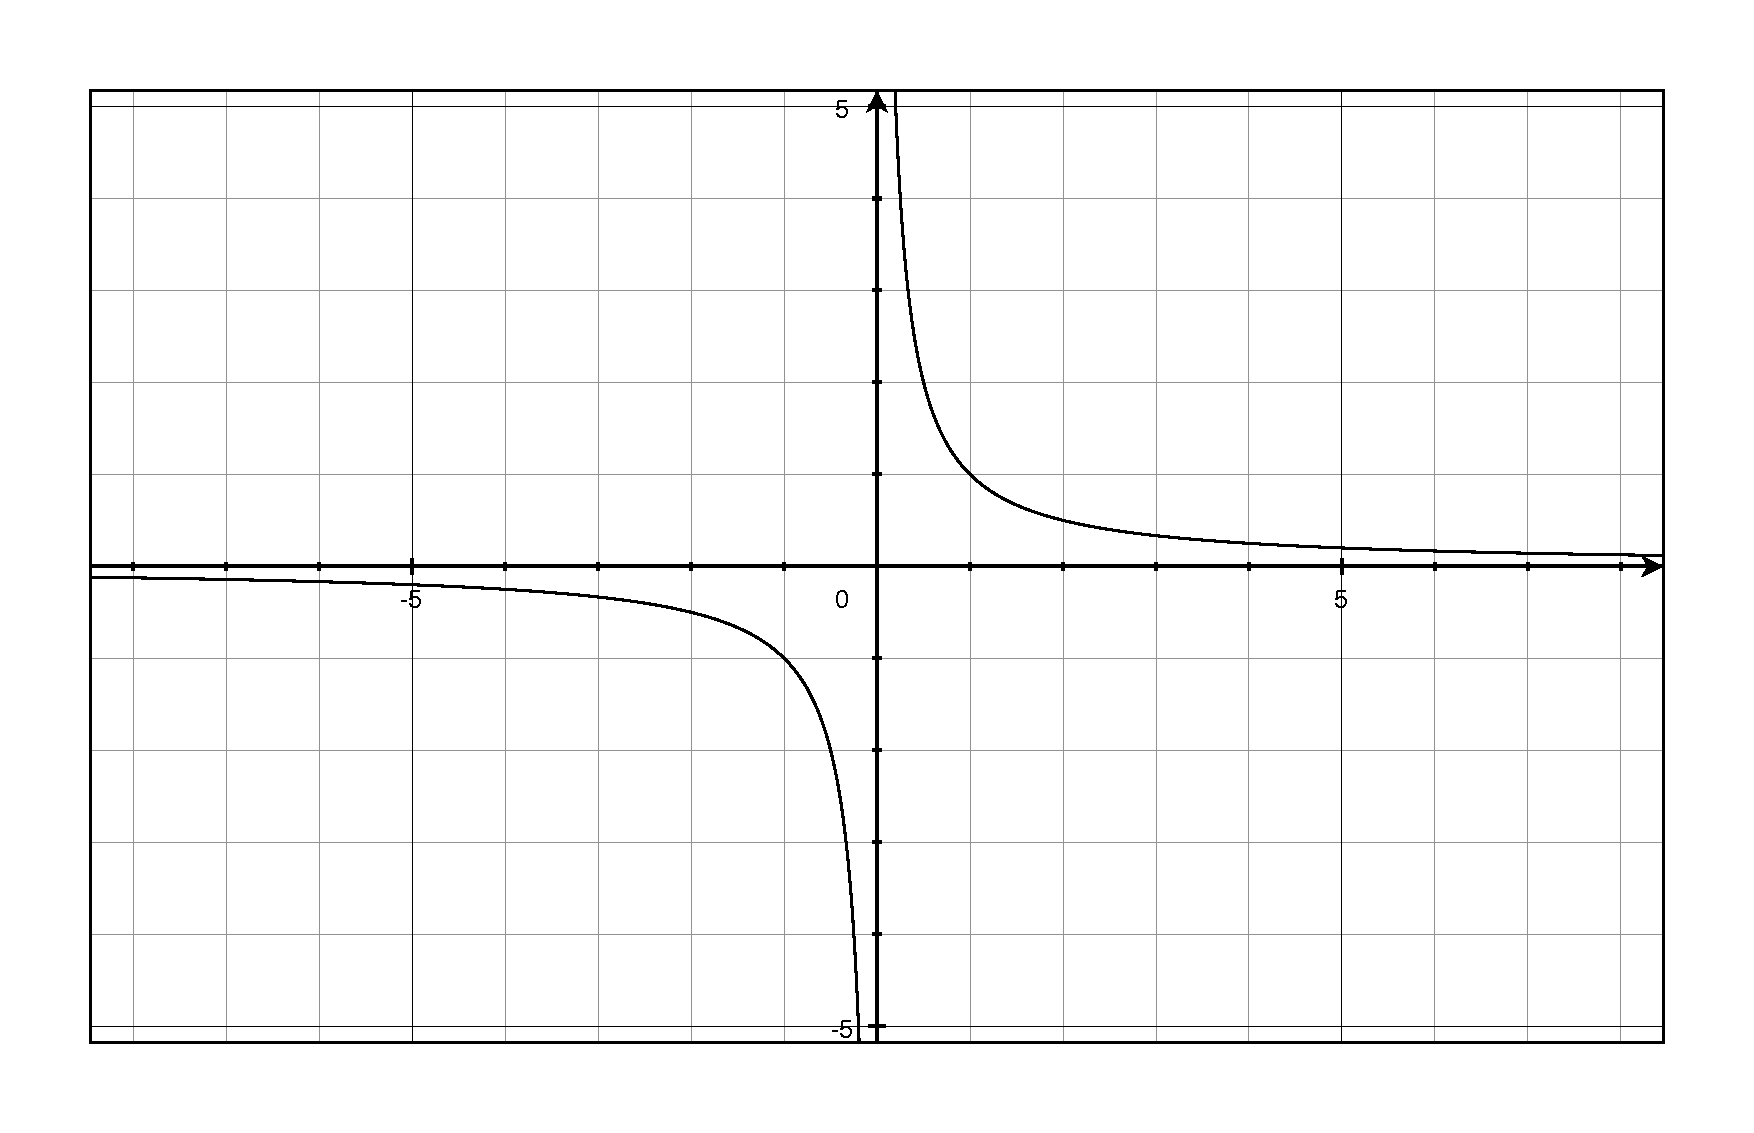
\includegraphics[scale=.3]{problem_21a.eps}
            \caption*{Problem 21a: $f(x) = \frac{1}{x}$}
          \end{figure}

        \part
        \begin{parts}
          \part $g(x) = f(-x)$.  The graph is the original graph reflected around the y-axis.
            \begin{figure}[H]
              \centering
              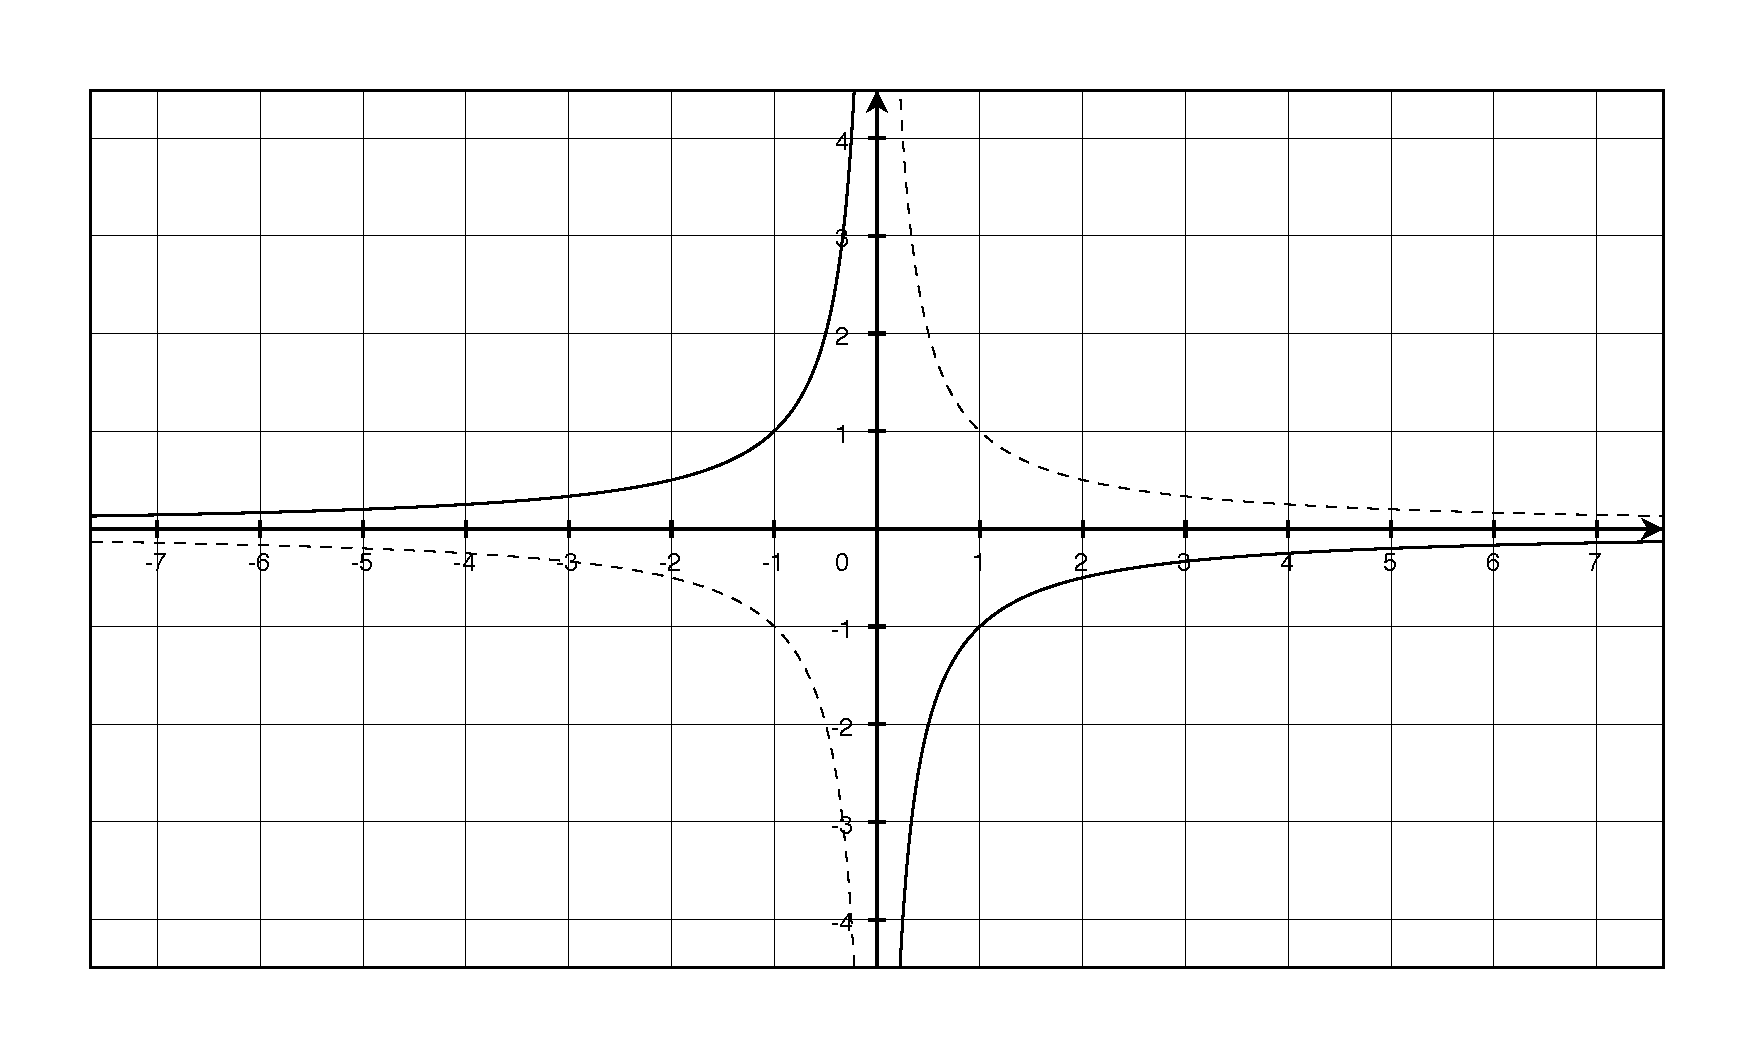
\includegraphics[scale=.3]{problem_21b_i.eps}
              \caption*{Problem 21b i: $f(-x)$}
            \end{figure}

          \part $g(x) = f(x - 1)$.  The graph is the original graph shifted right by 1.
            \begin{figure}[H]
              \centering
              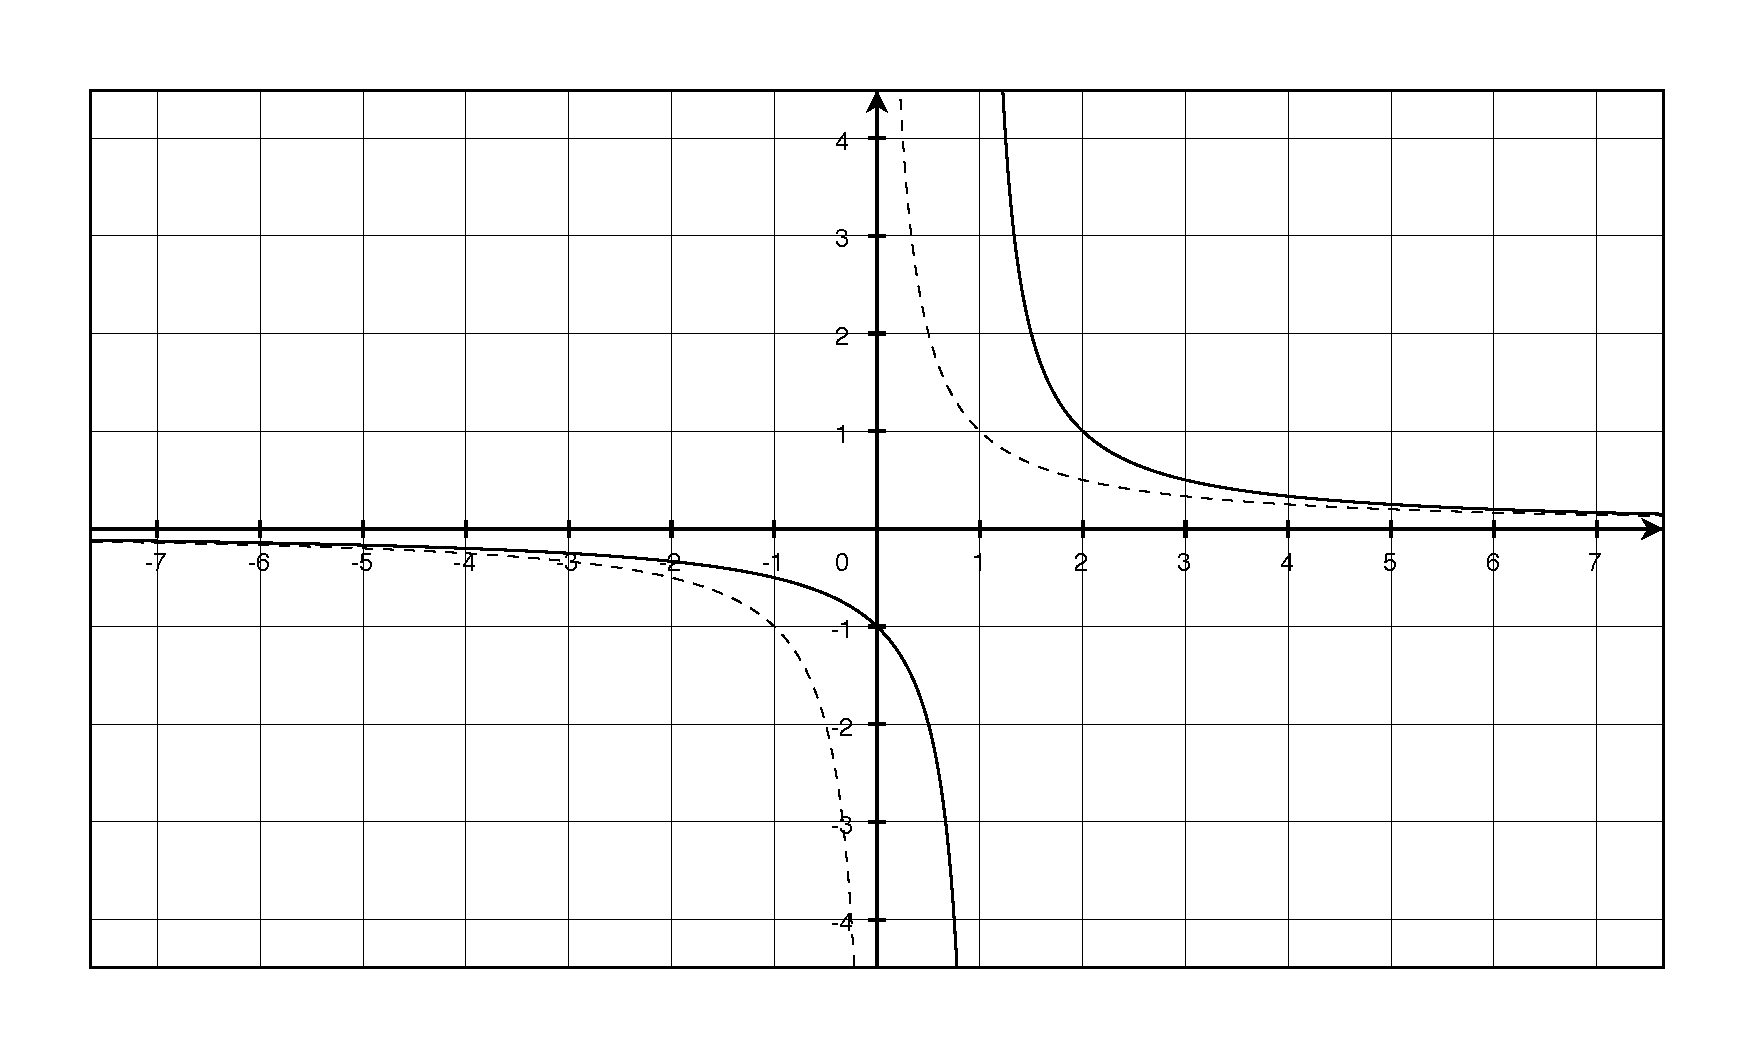
\includegraphics[scale=.3]{problem_21b_ii.eps}
              \caption*{Problem 21b ii: $f(x - 1)$}
            \end{figure}

          \part $g(x) = 2f(x + 2)$.  The graph is the original graph stretched vertically and shifted left 2.
            \begin{figure}[H]
              \centering
              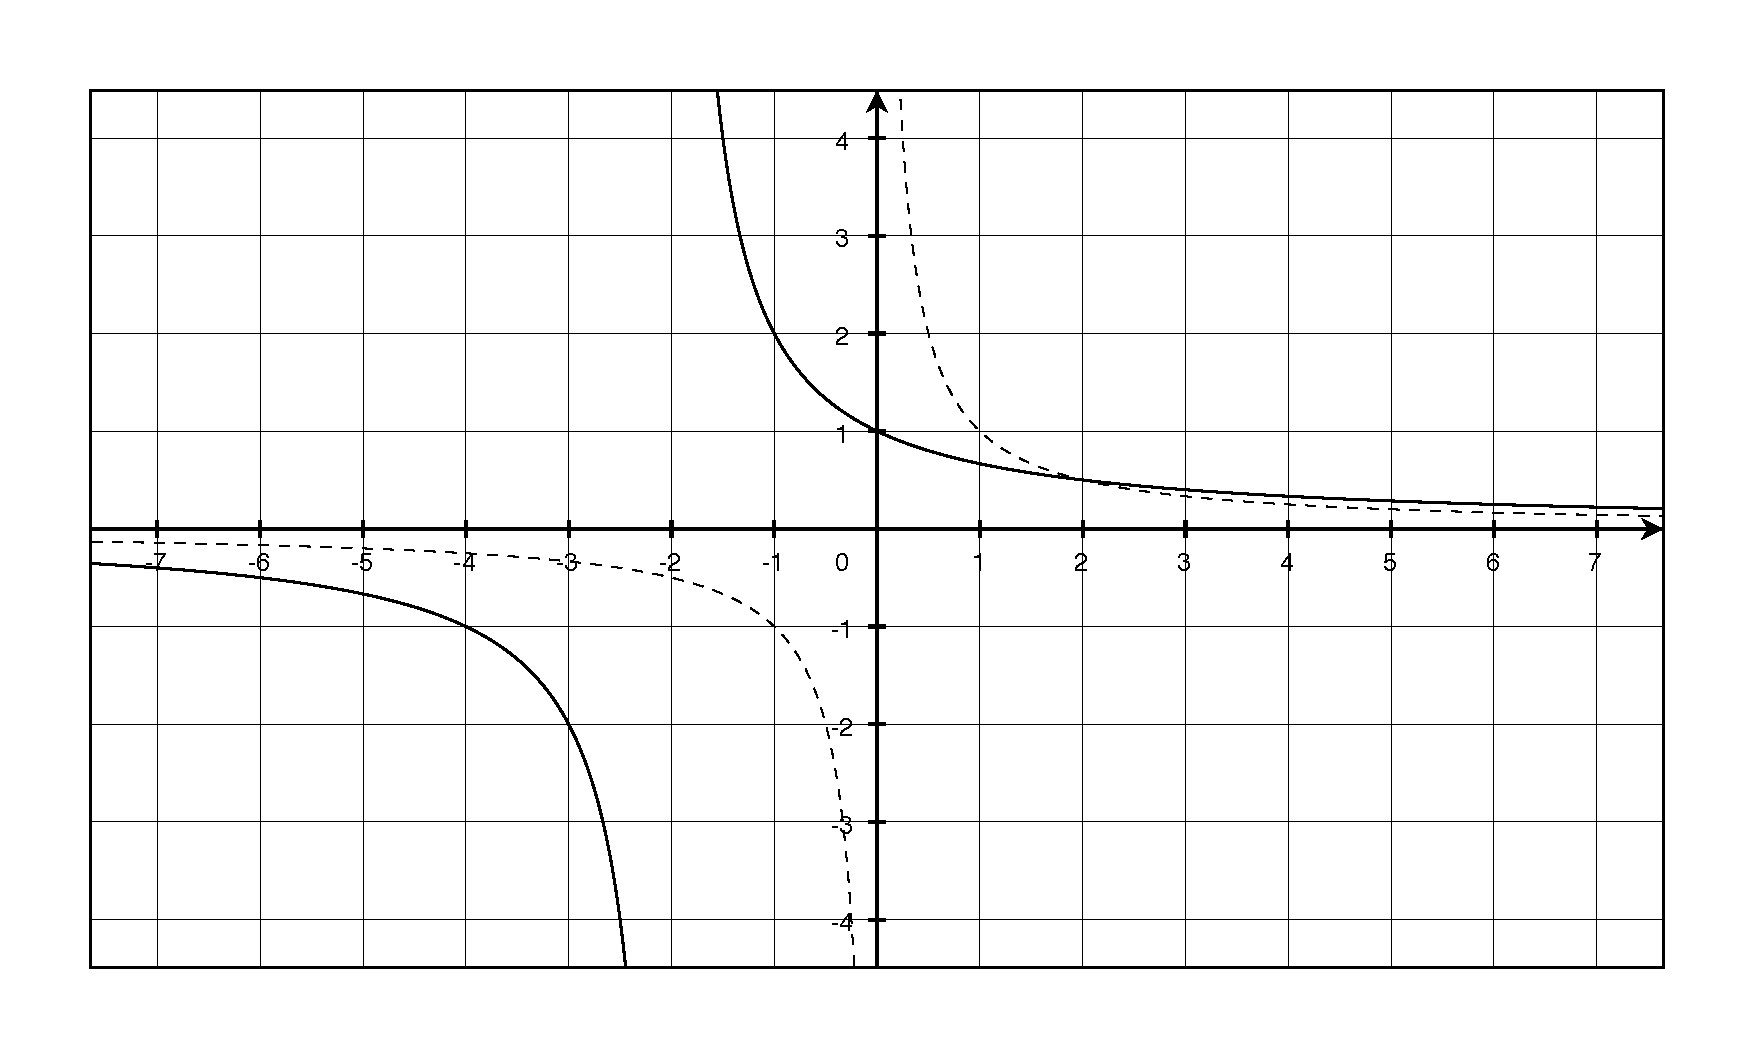
\includegraphics[scale=.3]{problem_21b_iii.eps}
              \caption*{Problem 21b iii: $2 f(x + 2)$}
            \end{figure}

          \part $g(x) = f(x - 3) + 1$.  The graph is the original graph shifted right 3 and up 1.
            \begin{figure}[H]
              \centering
              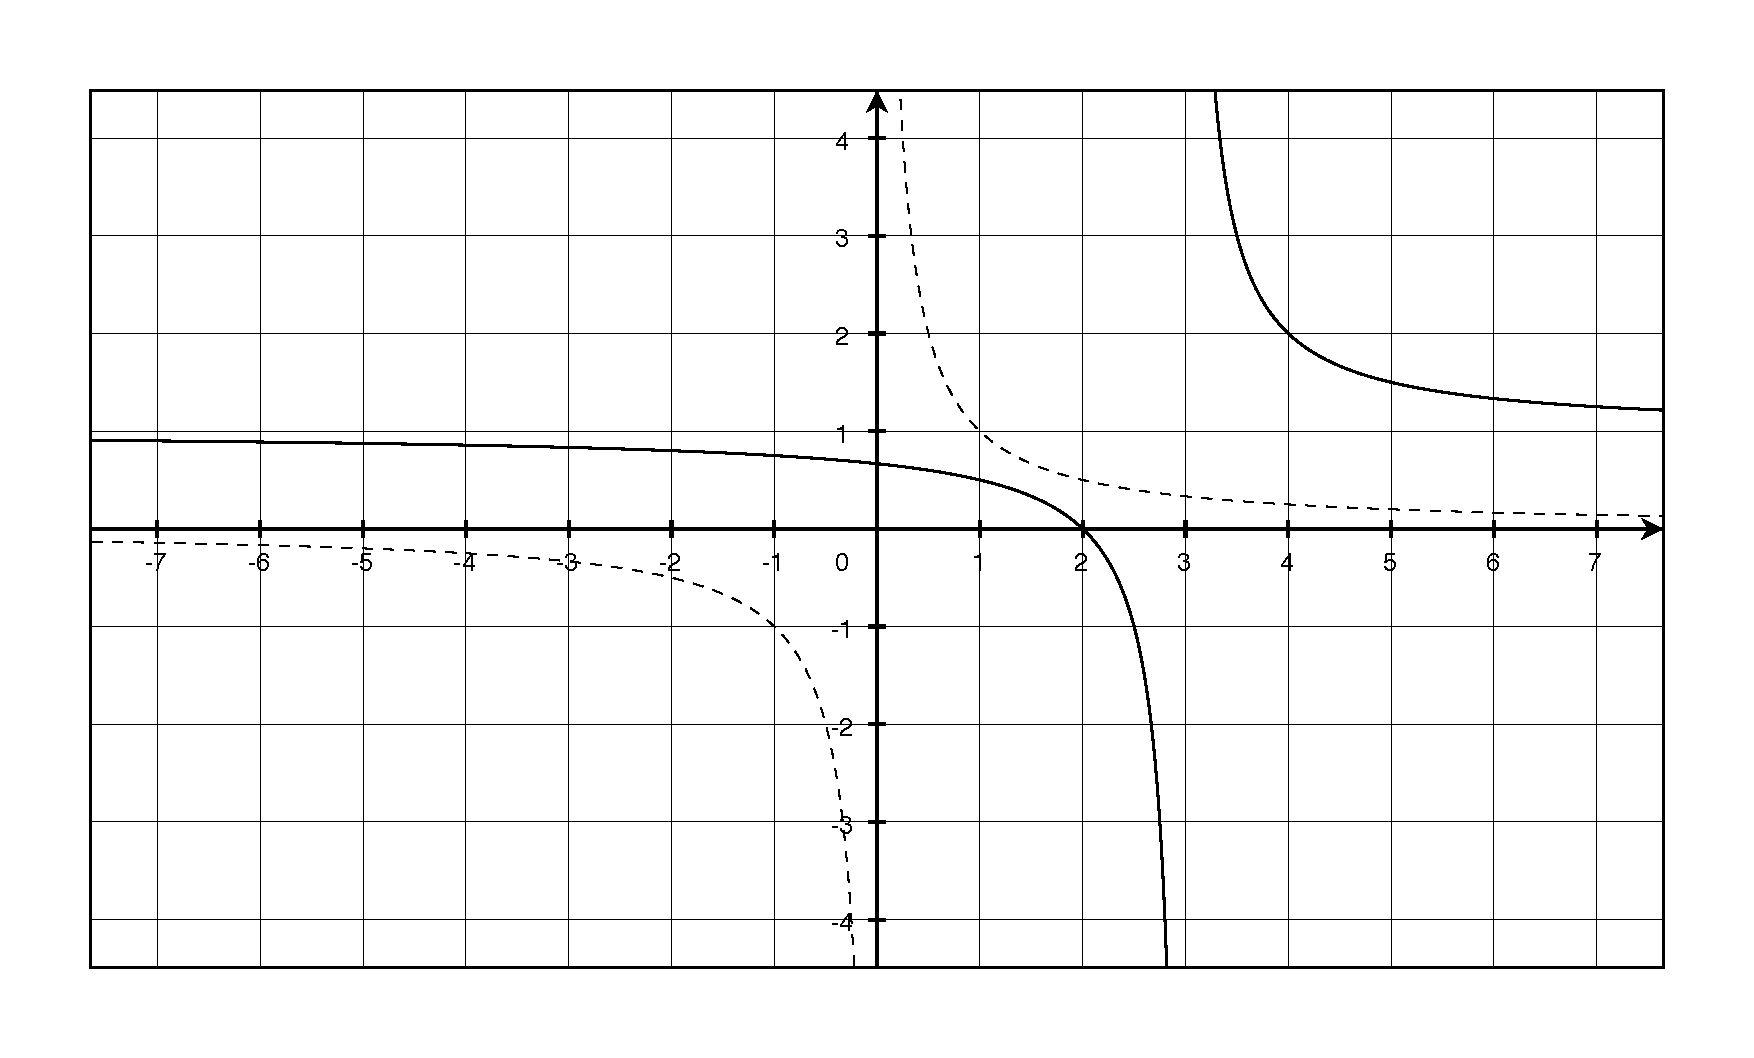
\includegraphics[scale=.3]{problem_21b_iv.eps}
              \caption*{Problem 21b iv: $g(x) = f(x - 3) + 1$}
            \end{figure}
        \end{parts}
      \end{parts}

    \item[27] $g(x) = (x - 2)^2 + 3$

    \item[28] $g(x) = (x + 4)^3 - 1$
      
    \item[29] $g(x) = -5 \sqrt{x + 3}$
      
    \item[30] $g(x) = \frac{1}{2} \cdot \sqrt[3]{-x} + \frac{3}{5}$

    \item[31] $g(x) = 0.1 \cdot \left| x - \frac{1}{2} \right| - 2$
      
    \item[32] $g(x) = 3 \cdot |x + 1| + 10$
      
    \item[33]
      \begin{figure}[H]
        \centering
        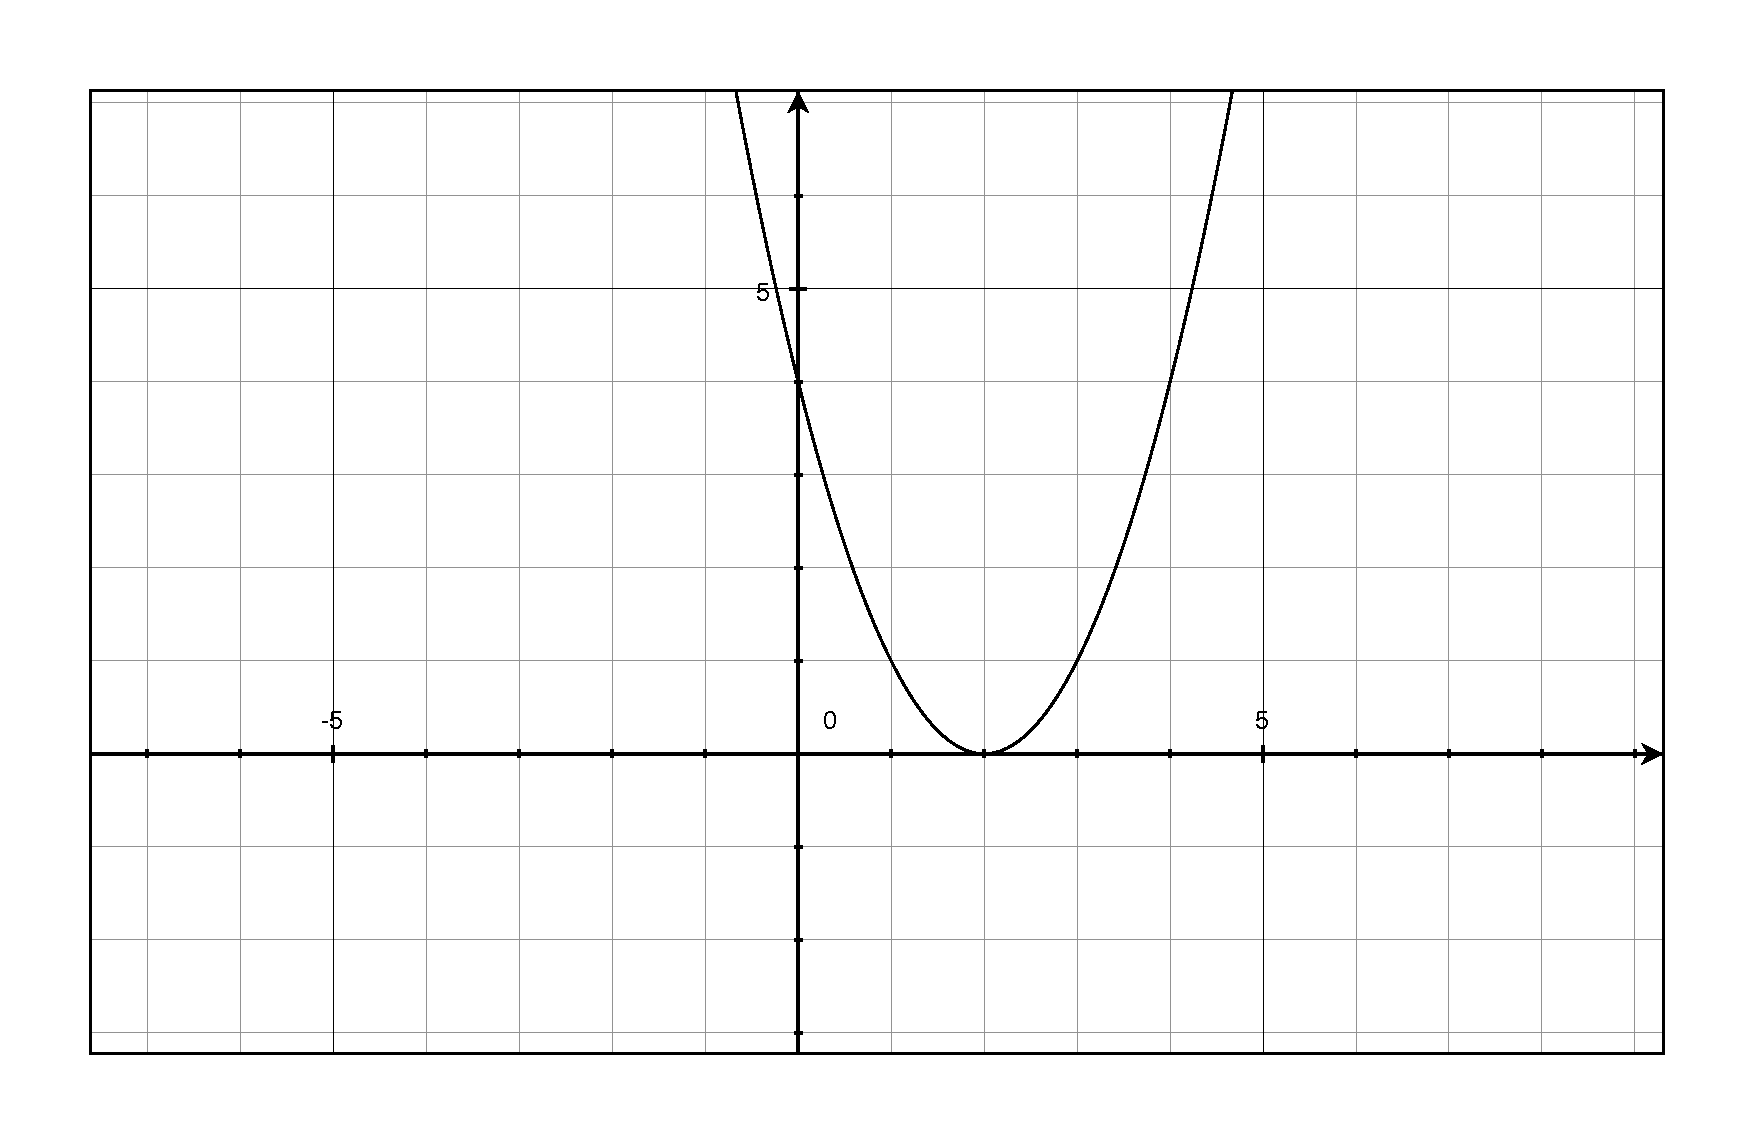
\includegraphics[scale=.3]{problem_33.eps}
        \caption*{Problem 33: $f(x) = (x - 2)^2$}
      \end{figure}

    \item[34]
      \begin{figure}[H]
        \centering
        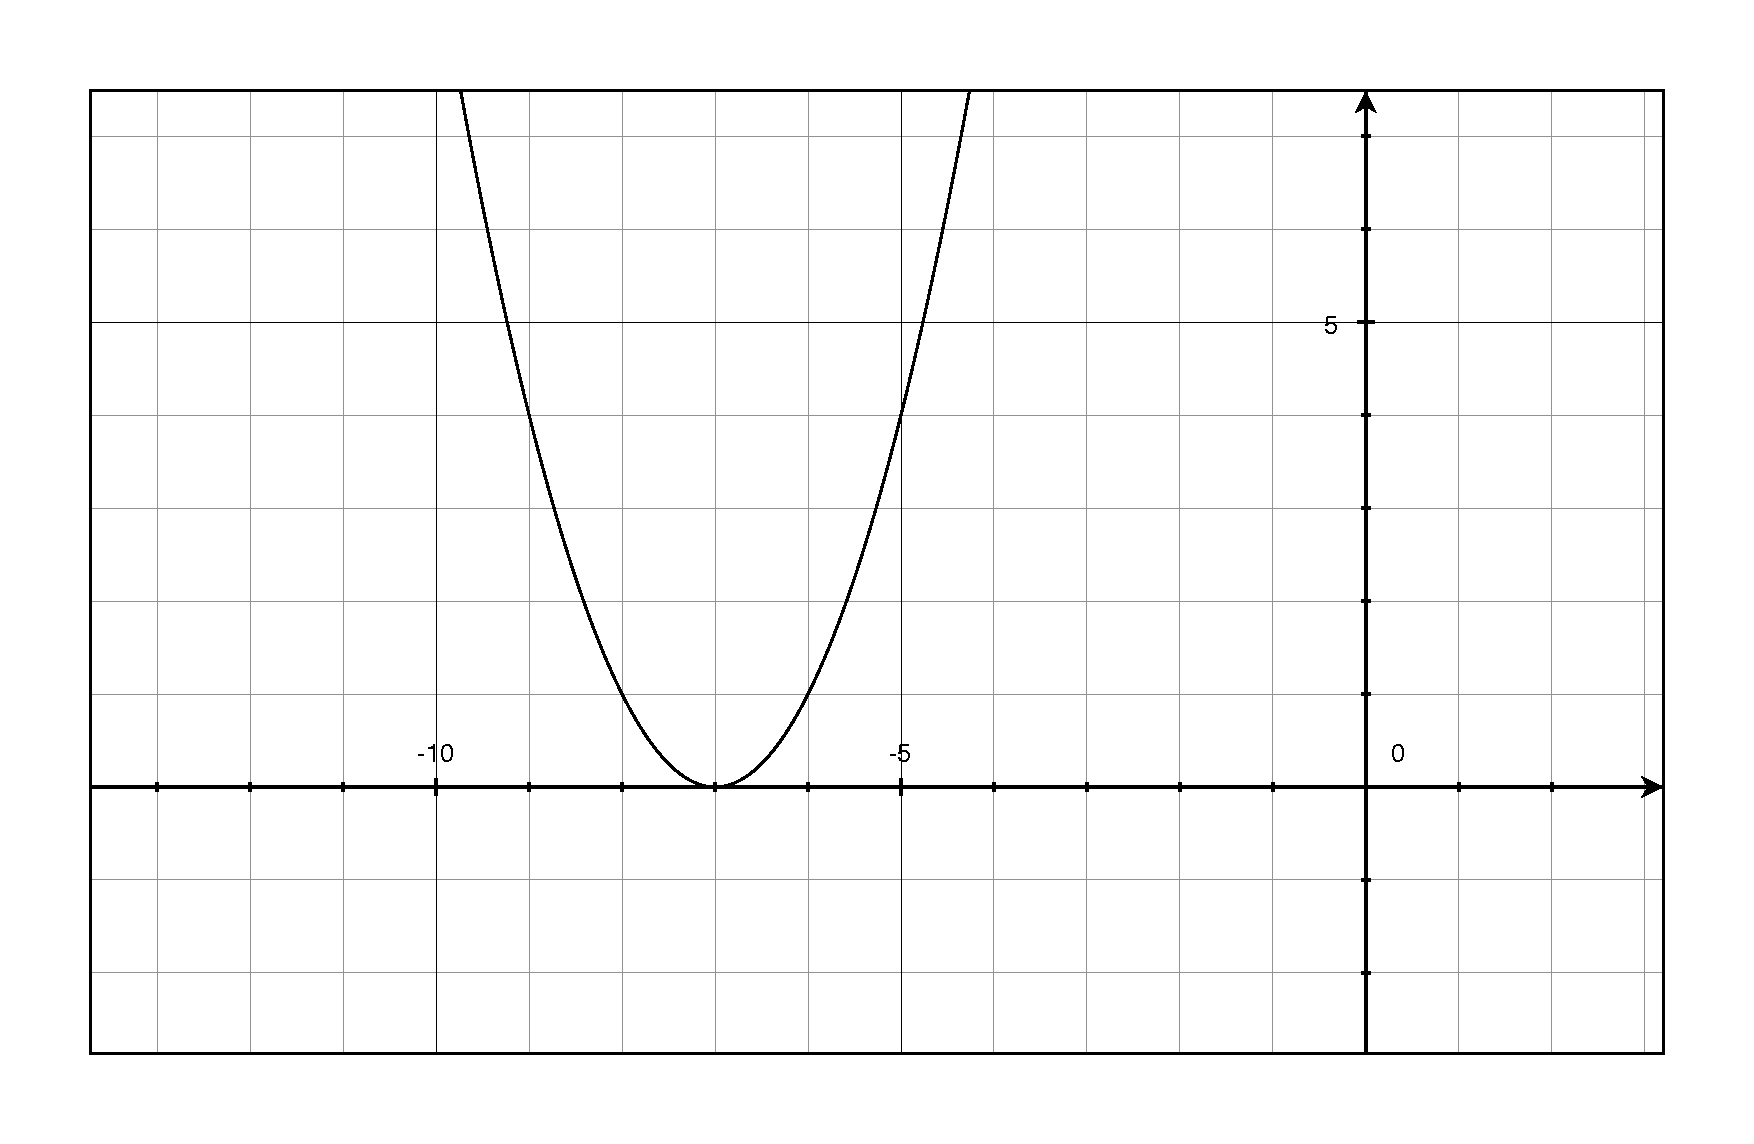
\includegraphics[scale=.3]{problem_34.eps}
        \caption*{Problem 34: $f(x) = (x + 7)^2$}
      \end{figure}

    \item[35]
      \begin{figure}[H]
        \centering
        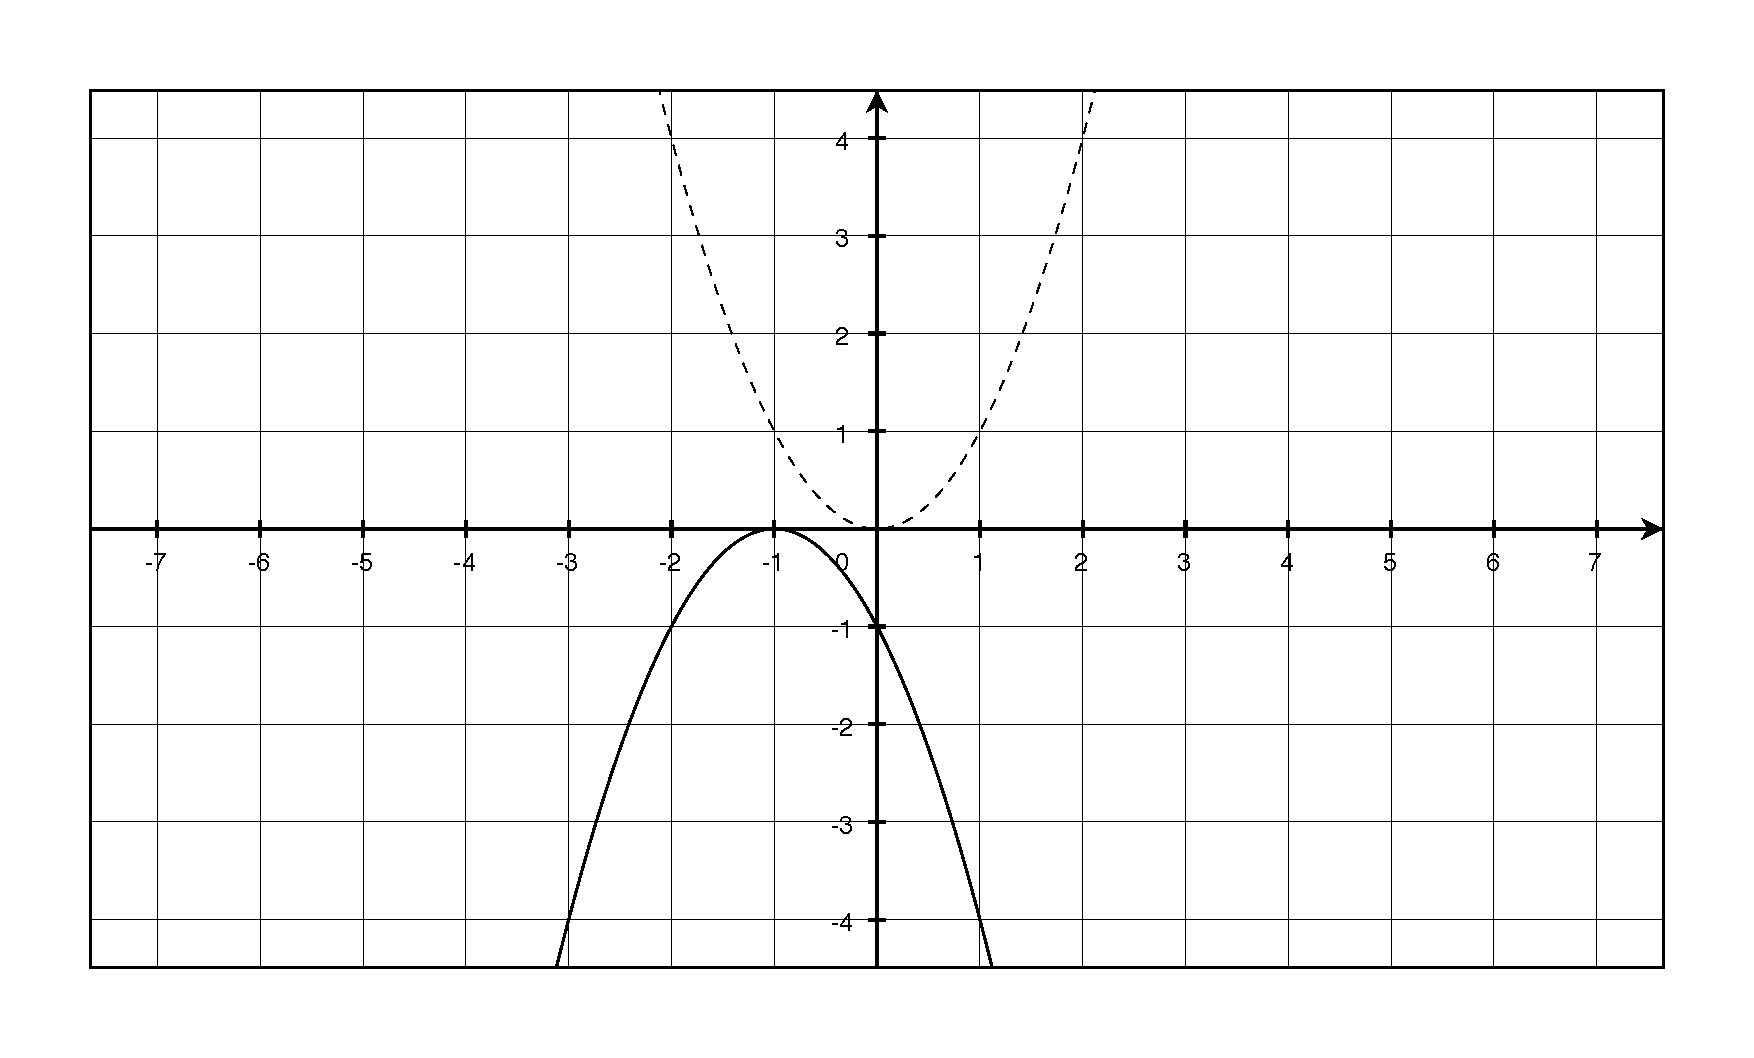
\includegraphics[scale=.3]{problem_35.eps}
        \caption*{Problem 35: $f(x) = -(x + 1)^2$}
      \end{figure}

    \item[36]
      \begin{figure}[H]
        \centering
        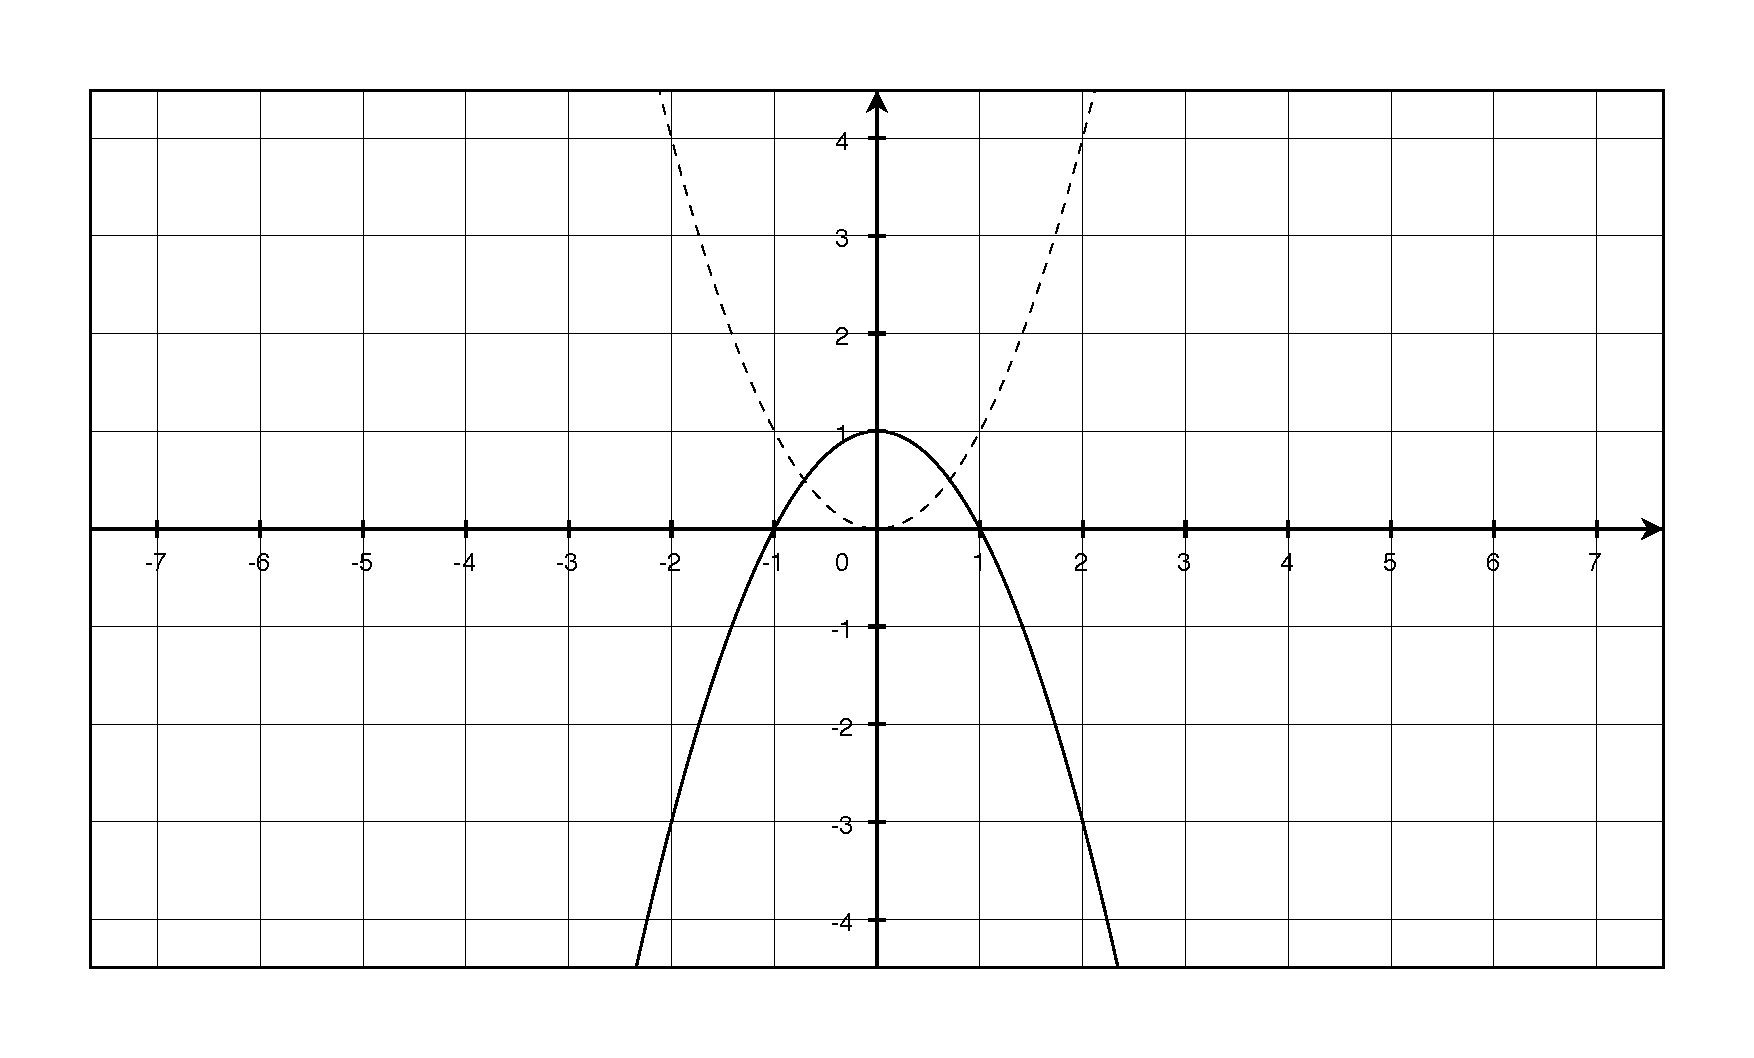
\includegraphics[scale=.3]{problem_36.eps}
        \caption*{Problem 36: $f(x) = 1 - x^2$}
      \end{figure}

    \item[37]
      \begin{figure}[H]
        \centering
        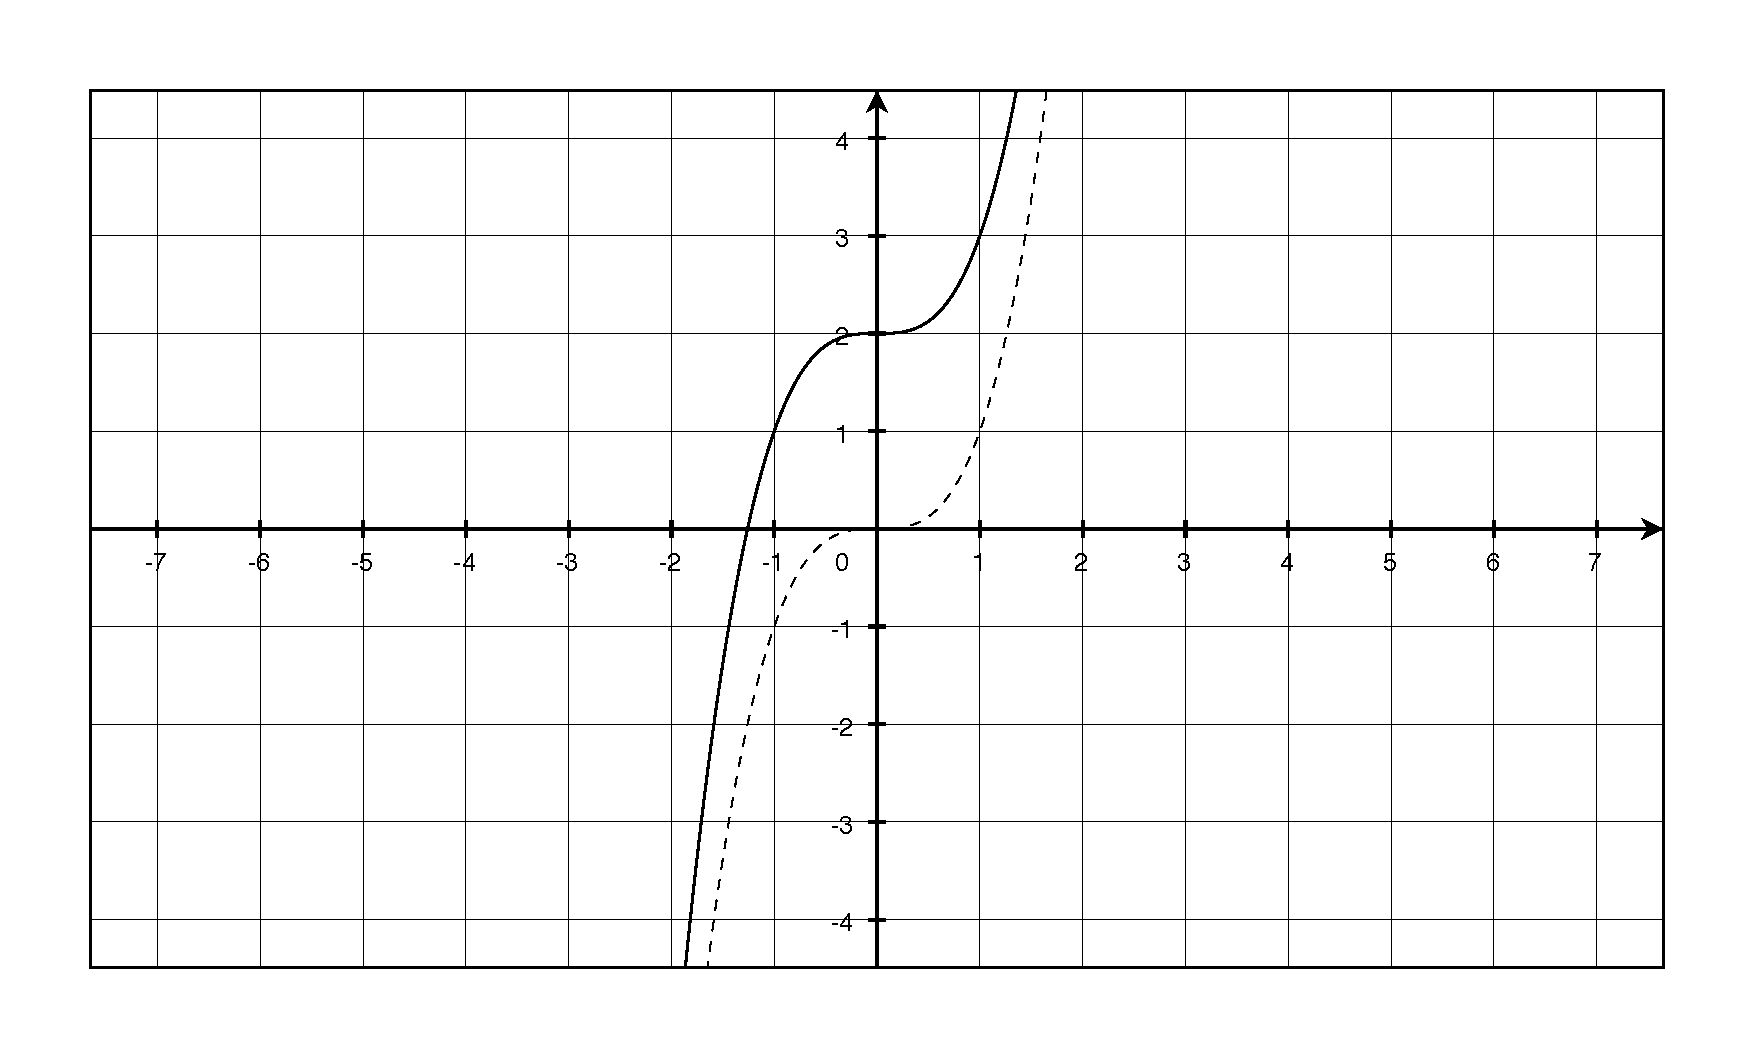
\includegraphics[scale=.3]{problem_37.eps}
        \caption*{Problem 37: $f(x) = x^3 + 2$}
      \end{figure}

    \item[38]
      \begin{figure}[H]
        \centering
        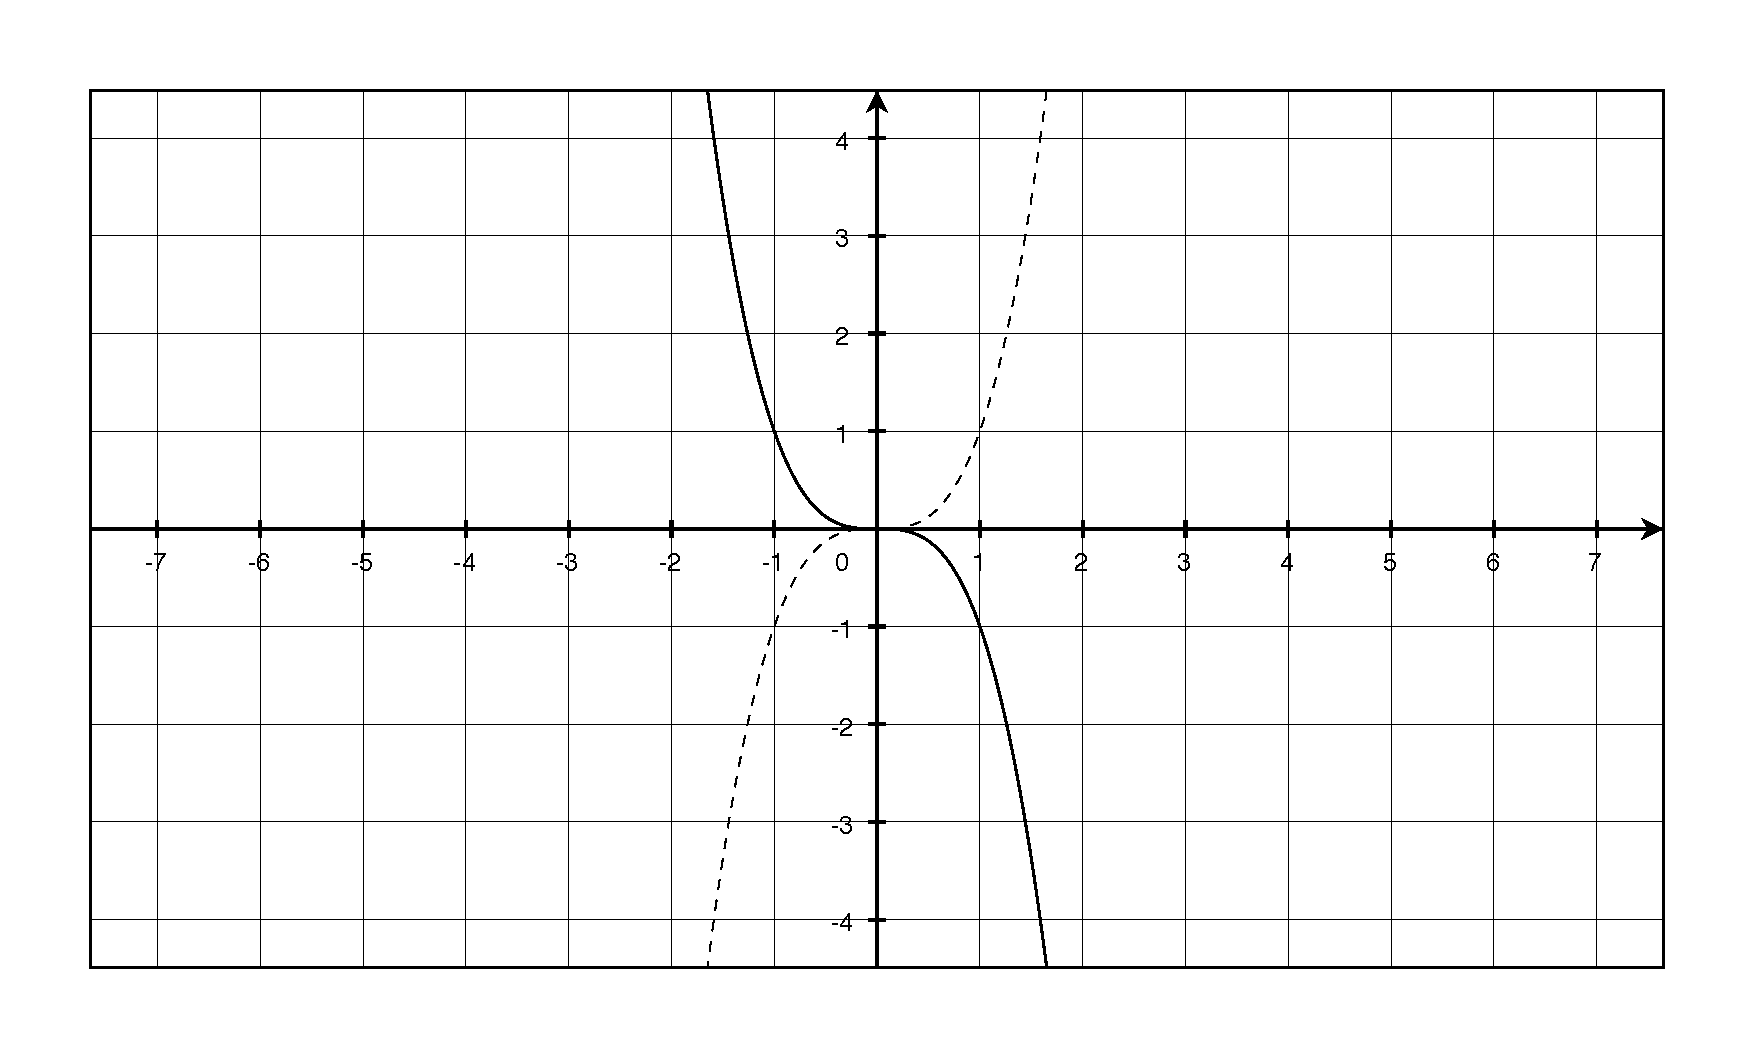
\includegraphics[scale=.3]{problem_38.eps}
        \caption*{Problem 38: $f(x) = -x^3$}
      \end{figure}

    \item[39]
      \begin{figure}[H]
        \centering
        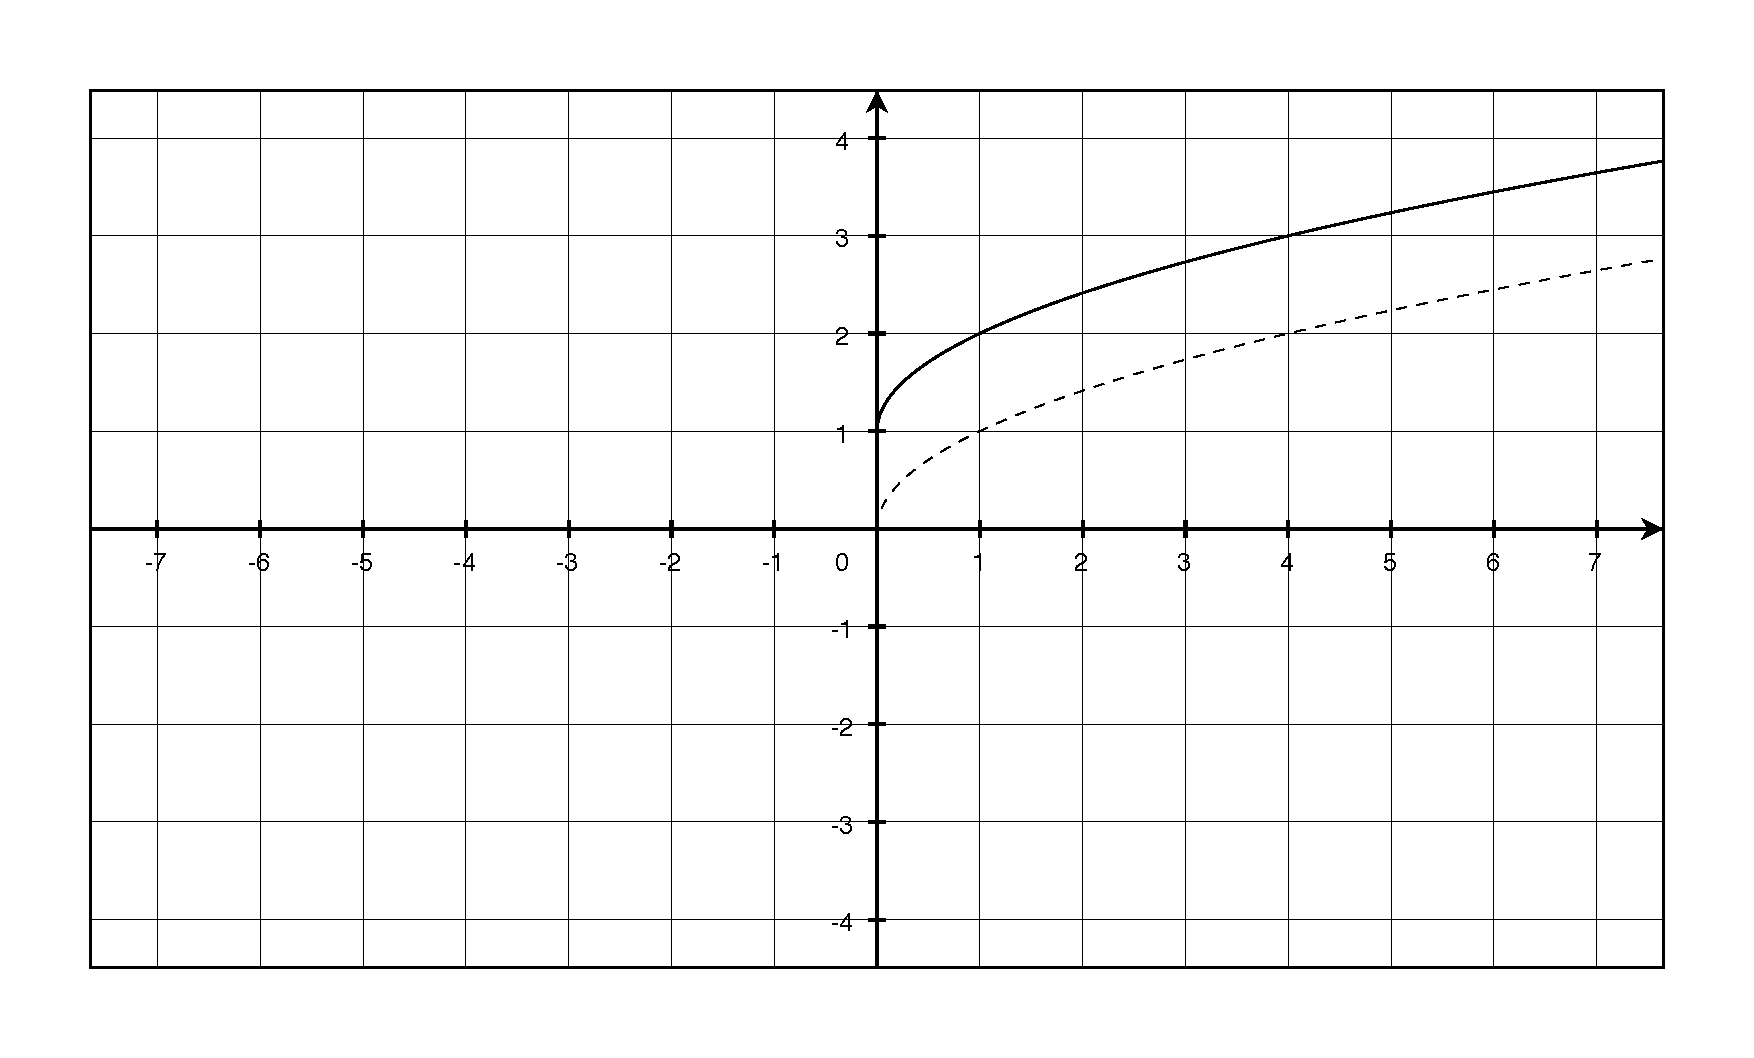
\includegraphics[scale=.3]{problem_39.eps}
        \caption*{Problem 39: $f(x) = 1 + \sqrt{x}$}
      \end{figure}

    \item[40]
      \begin{figure}[H]
        \centering
        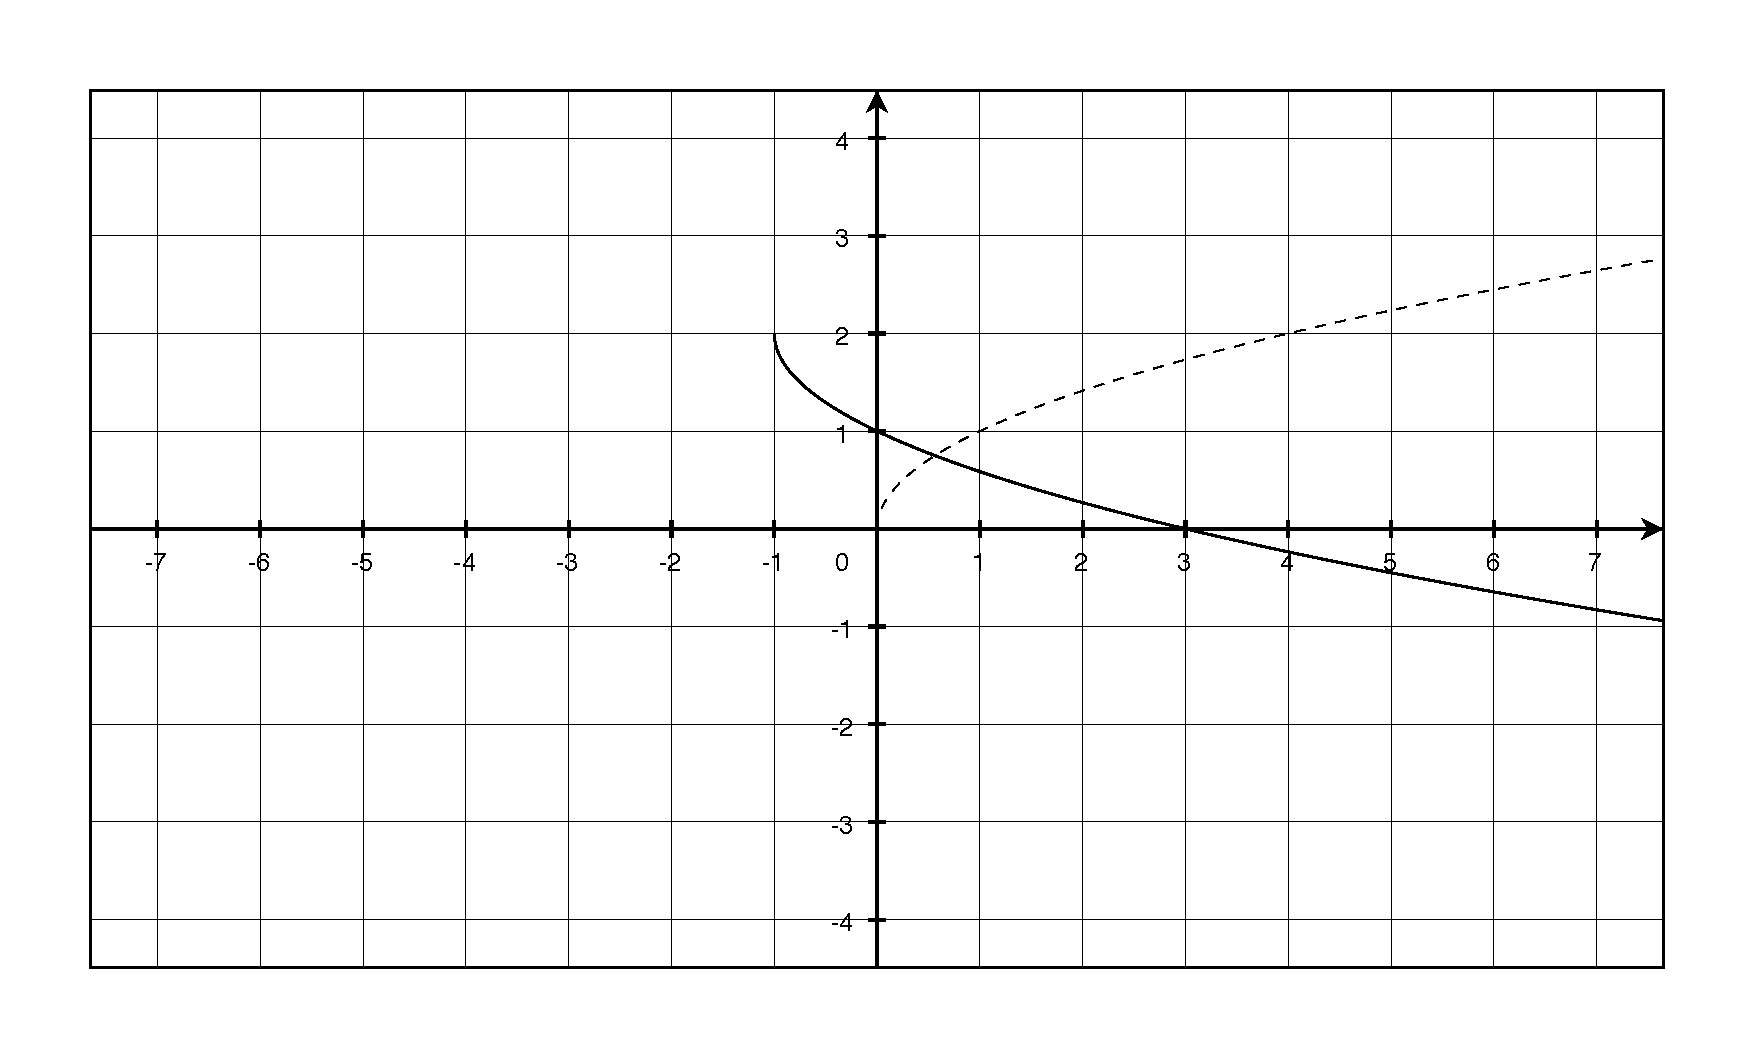
\includegraphics[scale=.3]{problem_40.eps}
        \caption*{Problem 40:  $f(x) = 2 - \sqrt{x + 1}$ }
      \end{figure}

    \item[47]
      \begin{figure}[H]
        \centering
        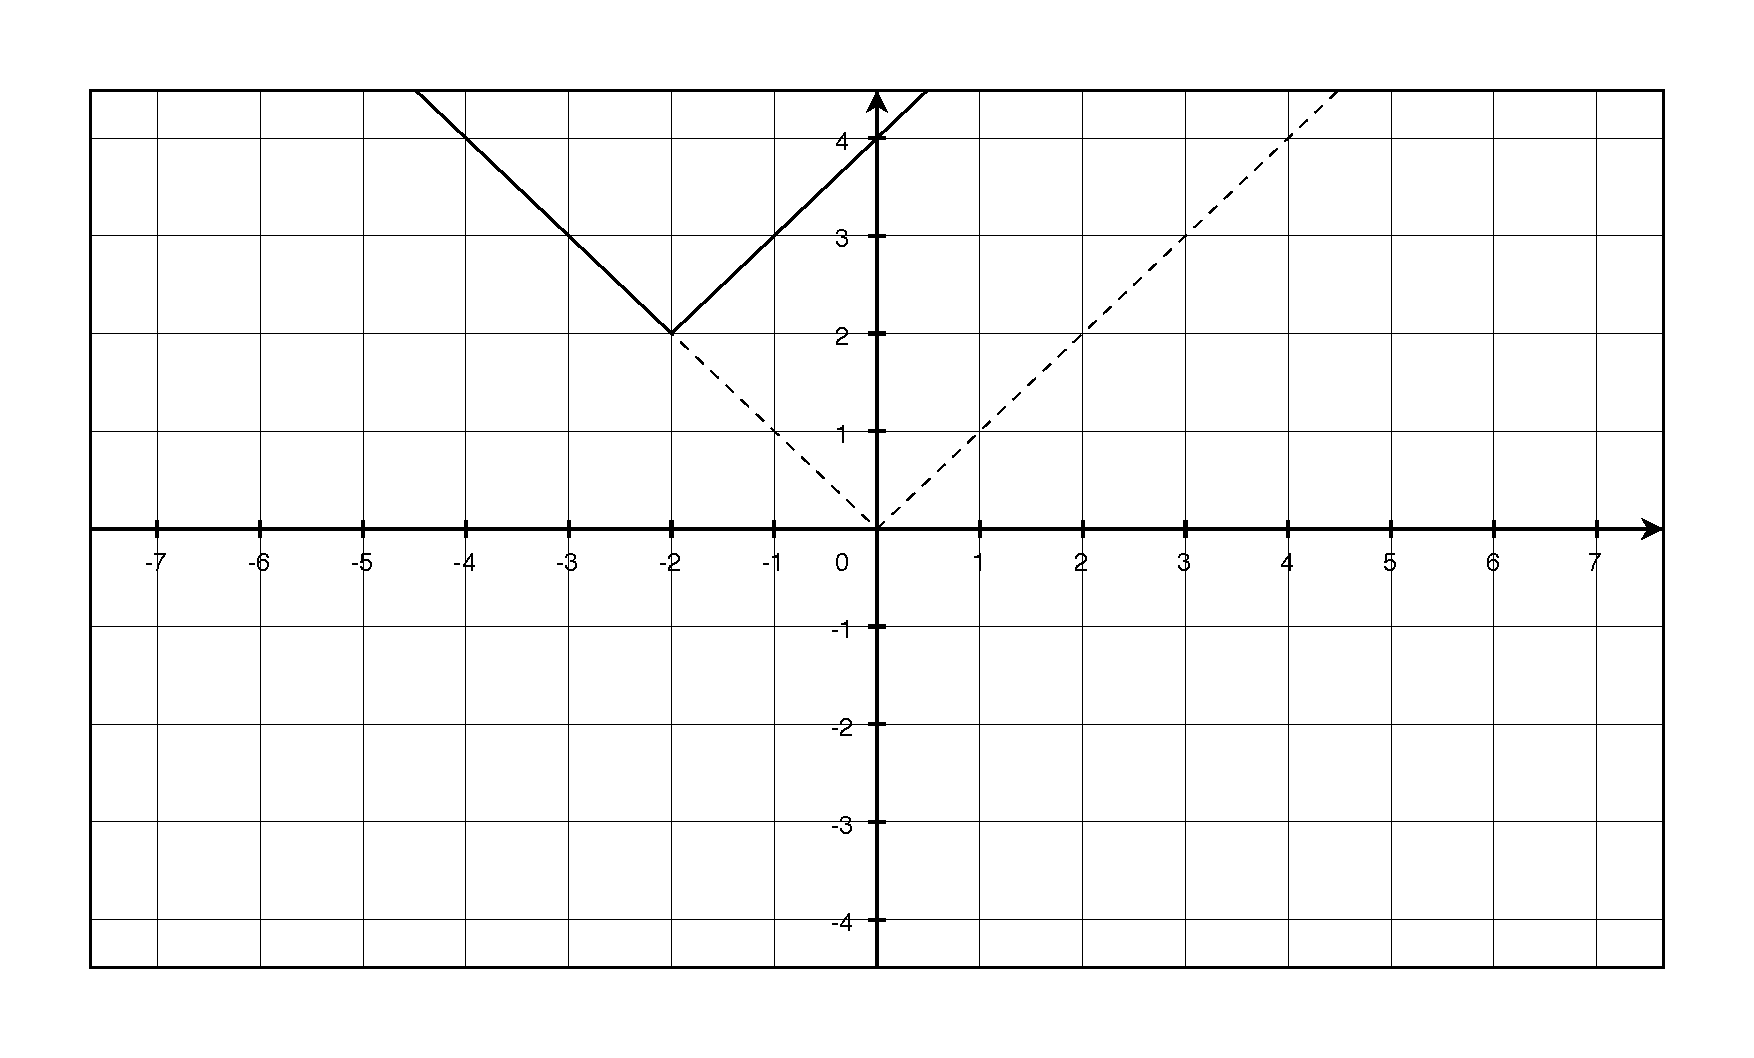
\includegraphics[scale=.3]{problem_47.eps}
        \caption*{Problem 47:  $f(x) = |x + 2| + 2$ }
      \end{figure}

    \item[48]
      \begin{figure}[H]
        \centering
        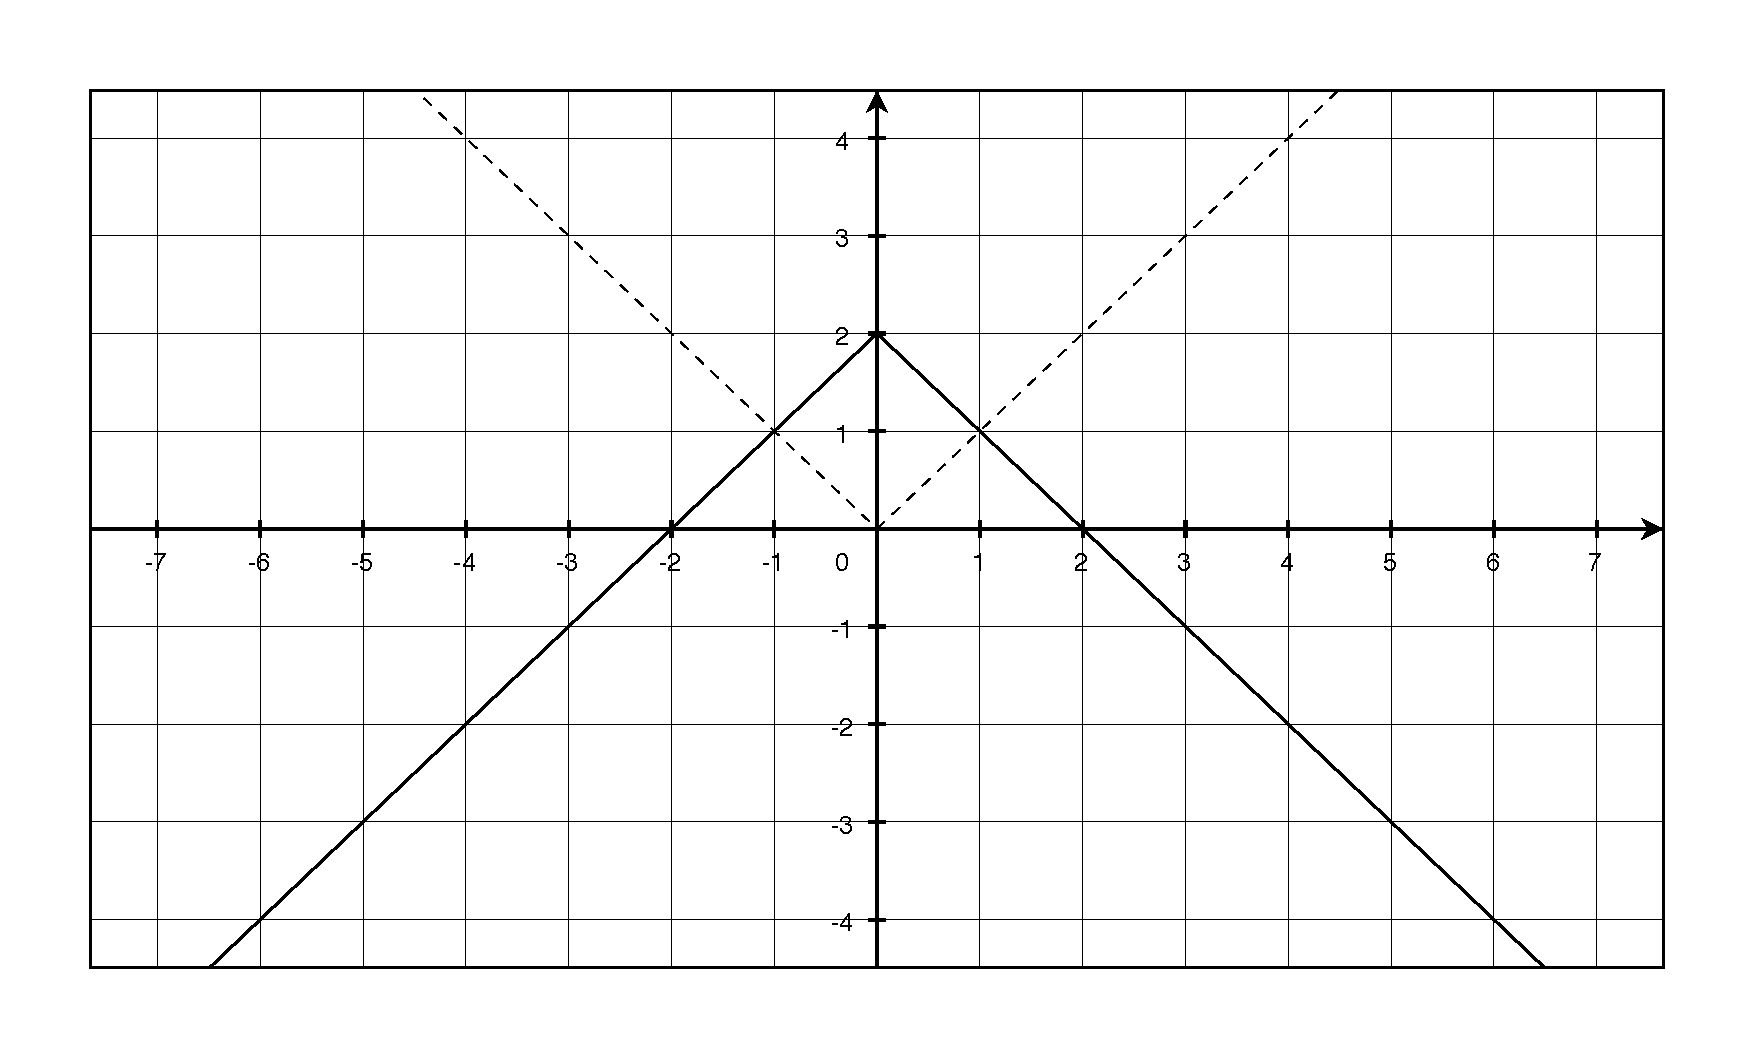
\includegraphics[scale=.3]{problem_48.eps}
        \caption*{Problem 48:  $f(x) = 2 - |x|$ }
      \end{figure}

    \item[61]
      \begin{align*}
        f(x)  &= \frac{1}{x^2} \\
        f(-x) &= \frac{1}{(-x)^2} \\ 
          &= \frac{1}{x^2} \\ 
          &= f(x) \\
      \end{align*}
      Since $f(x) = f(-x)$, this is an even function.

      \begin{figure}[H]
        \centering
        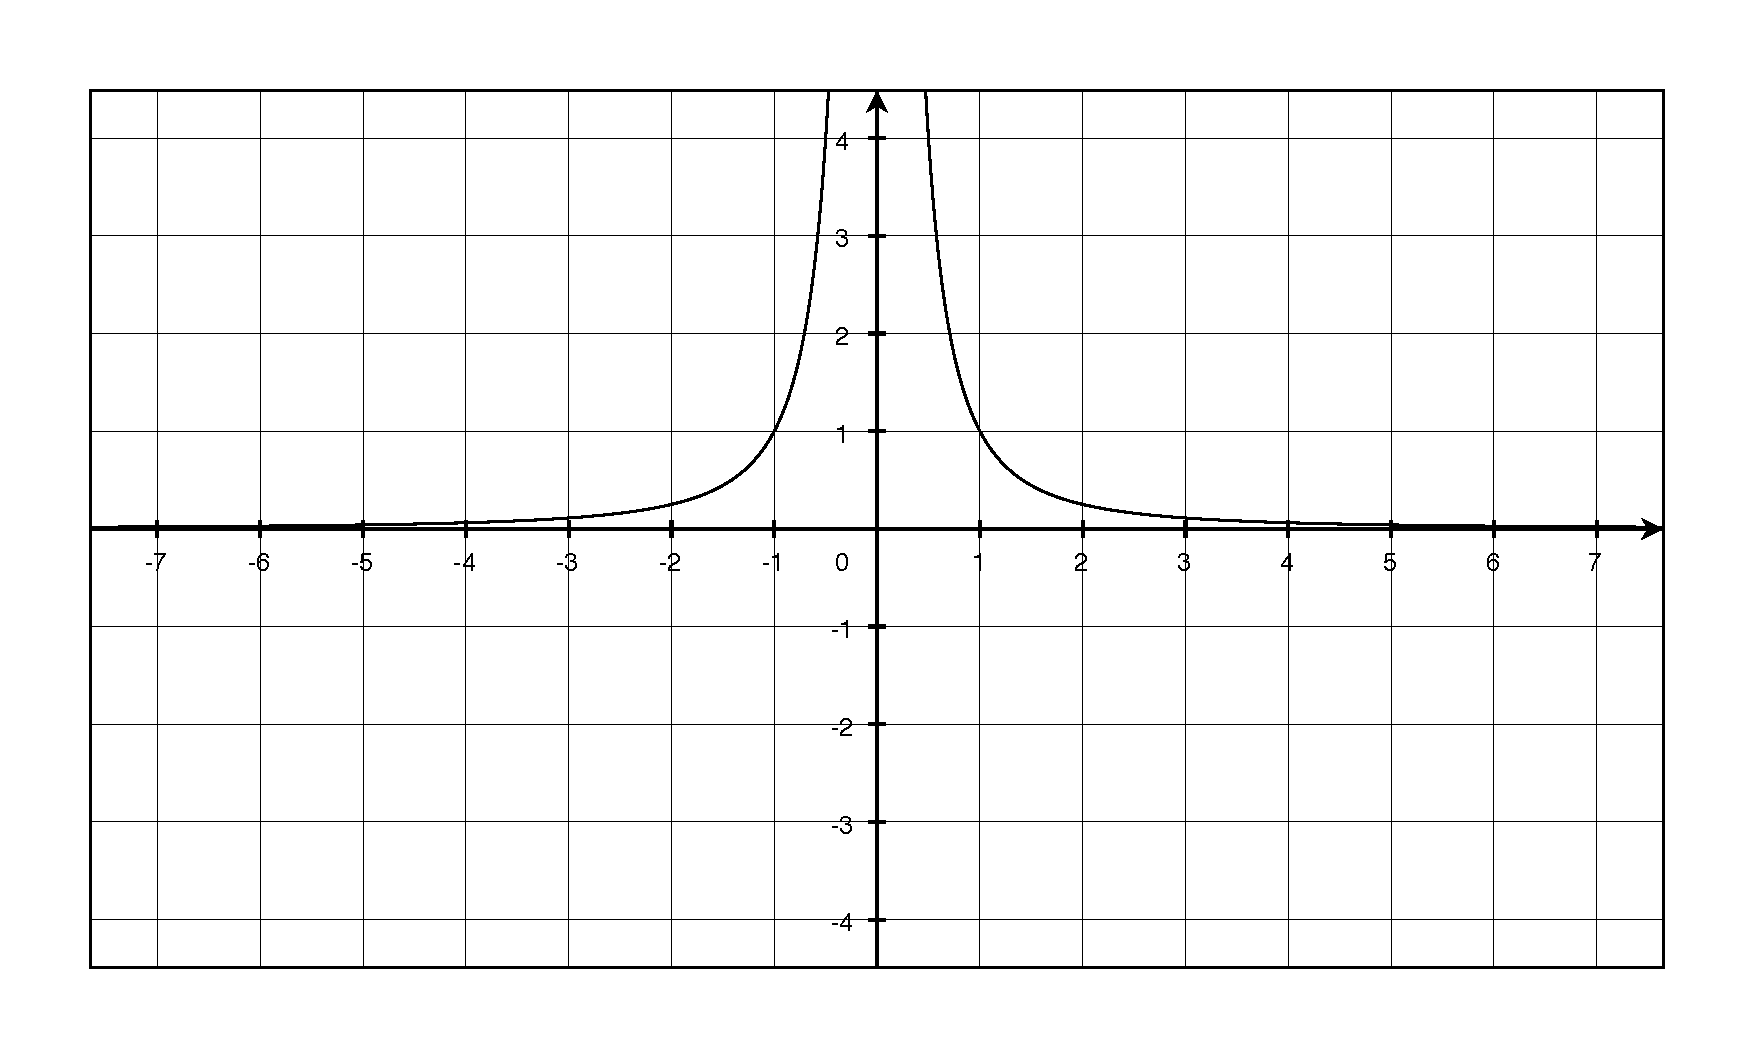
\includegraphics[scale=.3]{problem_61.eps}
        \caption*{Problem 61:  $f(x) = x^{-2}$ }
      \end{figure}

    \item[62]
      \begin{align*}
        f(x)  &= \frac{1}{x^3} \\
        f(-x) &= \frac{1}{(-x)^3} \\ 
          &= - \frac{1}{x^3} \\ 
          &= -f(x) \\
      \end{align*}
      Since $f(x) = -f(-x)$, this is an odd function.

      \begin{figure}[H]
        \centering
        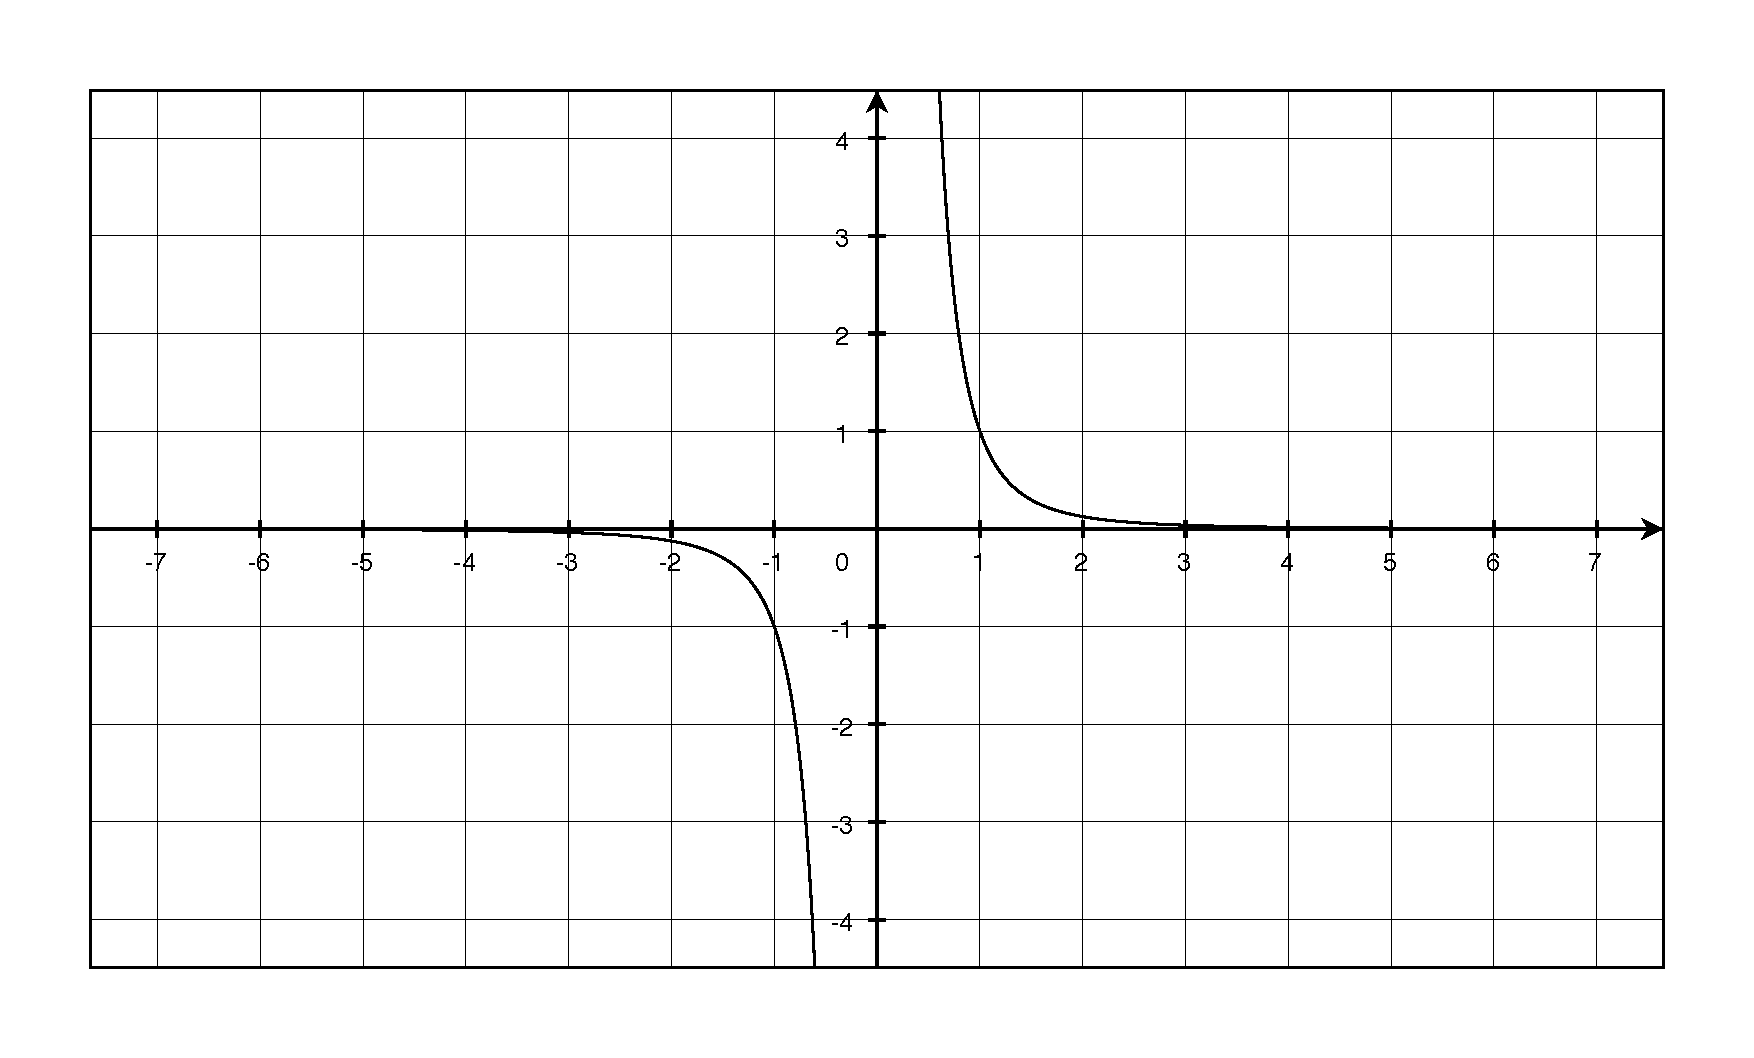
\includegraphics[scale=.3]{problem_62.eps}
        \caption*{Problem 62:  $f(x) = x^{-3}$ }
      \end{figure}

    \item[63]
      \begin{align*}
        f(x)  &= x^2 + x \\
        f(-x) &= (-x)^2 + (-x) \\
          &= x^2 - x \\
      \end{align*}
      Since $f(x) \neq f(-x)$ and $f(x) \neq -f(-x)$, this function is neither even nor odd.

    \item[69]
      Reflect all the negative values in the x-axis.
      
    \pagebreak

    \item[70]
      \begin{figure}[H]
        \centering
        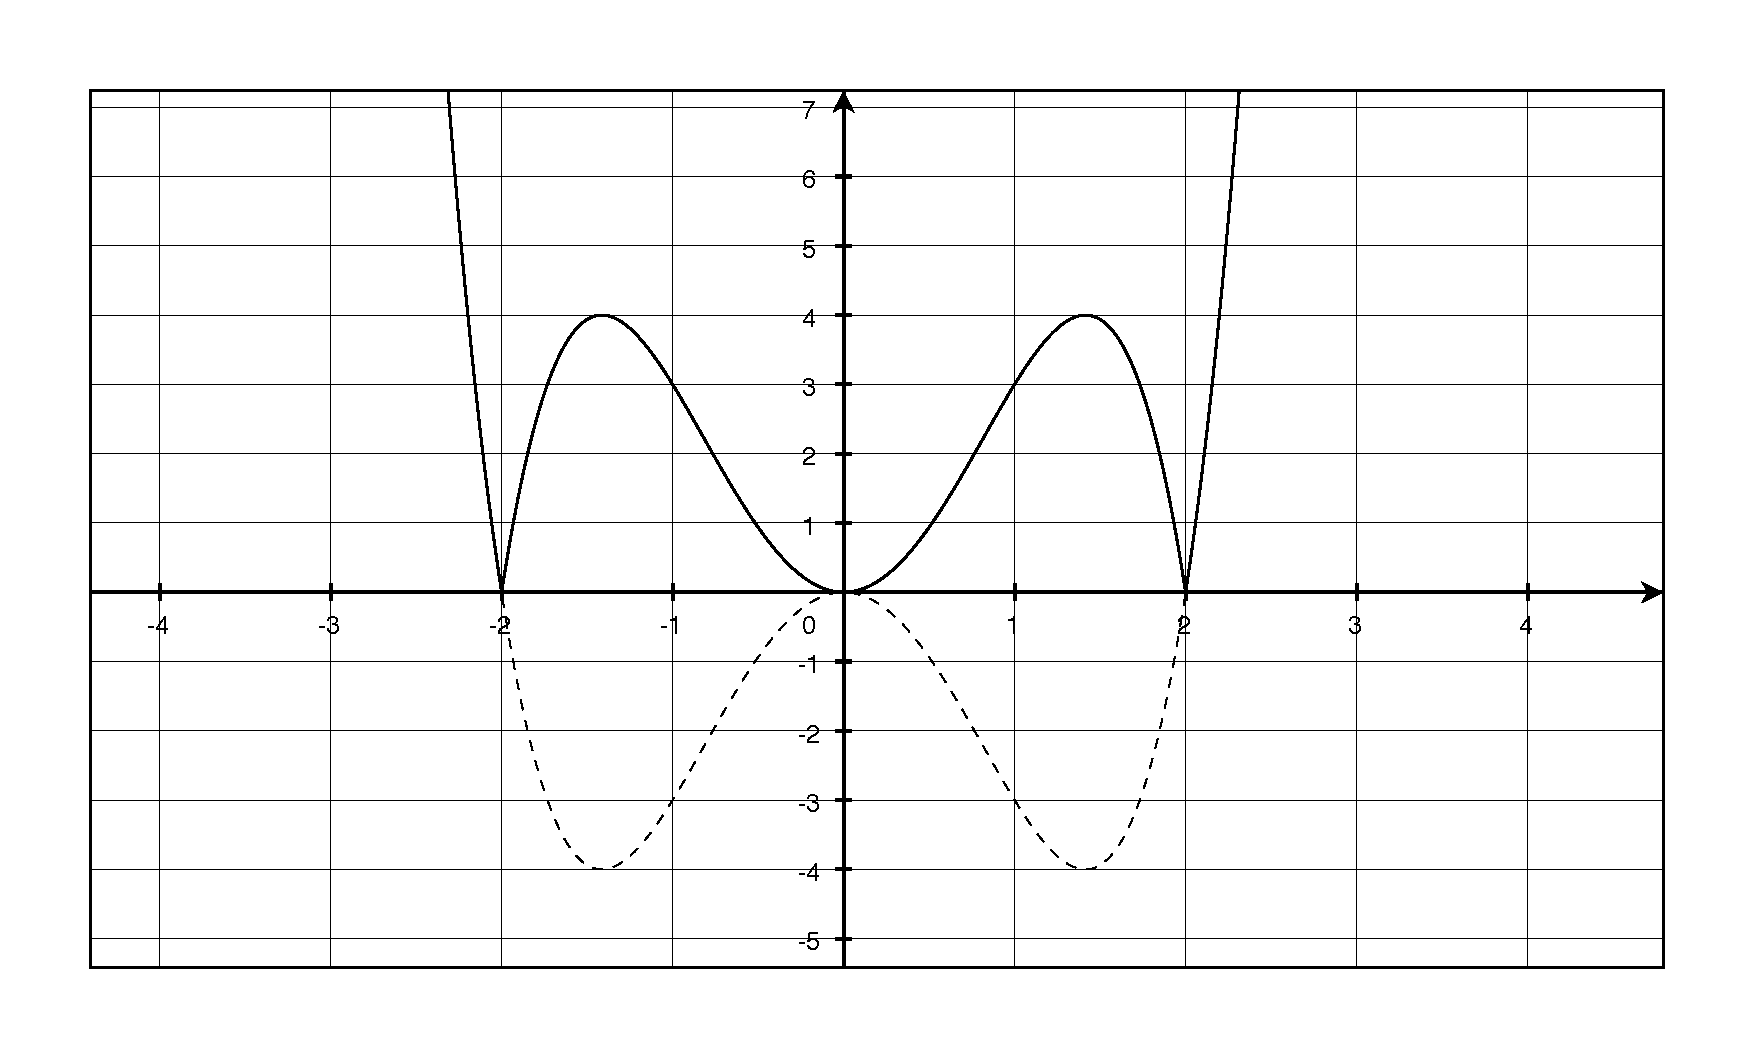
\includegraphics[scale=.3]{problem_70.eps}
        \caption*{Problem 70:  $f(x) = |x^4 - 4x^2|$ }
      \end{figure}

    \item[73]
      \begin{parts}
        \part Shift up 4 and shrink vertically by 0.01.
        \part Shift right by 10.  The new function would be: 
          \[
            g(t) = 4 + 0.01(t - 10)^2
          \]
      \end{parts}
  \end{description}
\else
  \vspace{9 cm}

  \emph{
    We are African, and we happened to be in America. We're not American. We are people who formerly were Africans who
    were kidnapped and brought to America. Our forefathers weren't the Pilgrims. We didn't land on Plymouth Rock. The
    rock was landed on us. We were brought here against our will. We were not brought here to be made citizens. We were
    not brought here to enjoy the constitutional gifts that they speak so beautifully about today.
  }

  \vspace{.2 cm}

  \hspace{1 cm} --Malcolm X

\fi

\end{document}

